%************************************************
\chapter{Spherical Brain Mapping}\label{ch:sbm}
%************************************************
\section{Introduction}
In this section we will deal with a feature extraction technique called \acf{SBM}. \ac{SBM} is based on the use of spherical coordinates to extract radial features from \ac{MRI} images, segmented. Using the features at each coordinate, we can characterize the texture in each direction, and even project the information to a bidimensional maps, which provides a significant feature reduction and a visual aid for diagnosis. 

The most basic form is the standard \ac{SBM} \cite{Martinez-Murcia2014225,Martinez-Murcia2015}, in which all voxels crossed by a rectilinear vector in a spherical coordinate pair ($\theta,\varphi$) are selected, and then, a certain measure is extracted from that set. In this sense, statistical and morphological measures such as tissue thickness, average or entropy, among others, are computed. 

Further improvements can be made to this simple approach, for example, with a layering extension \cite{Martinez-Murcia2015}, in which the mapping vector is divided in $n$ subsets containing the same number of voxels. Therefore, instead of a single map, we can obtain $n$ maps at different distances from the centre of the brain. Another useful approach is the characterization of texture features via \acf{LBP}, computed around the mapping vector, which yielded very good results in \cite{Martinez-MurciaVRLBP}.

\begin{figure*}[htp]
	\centering
	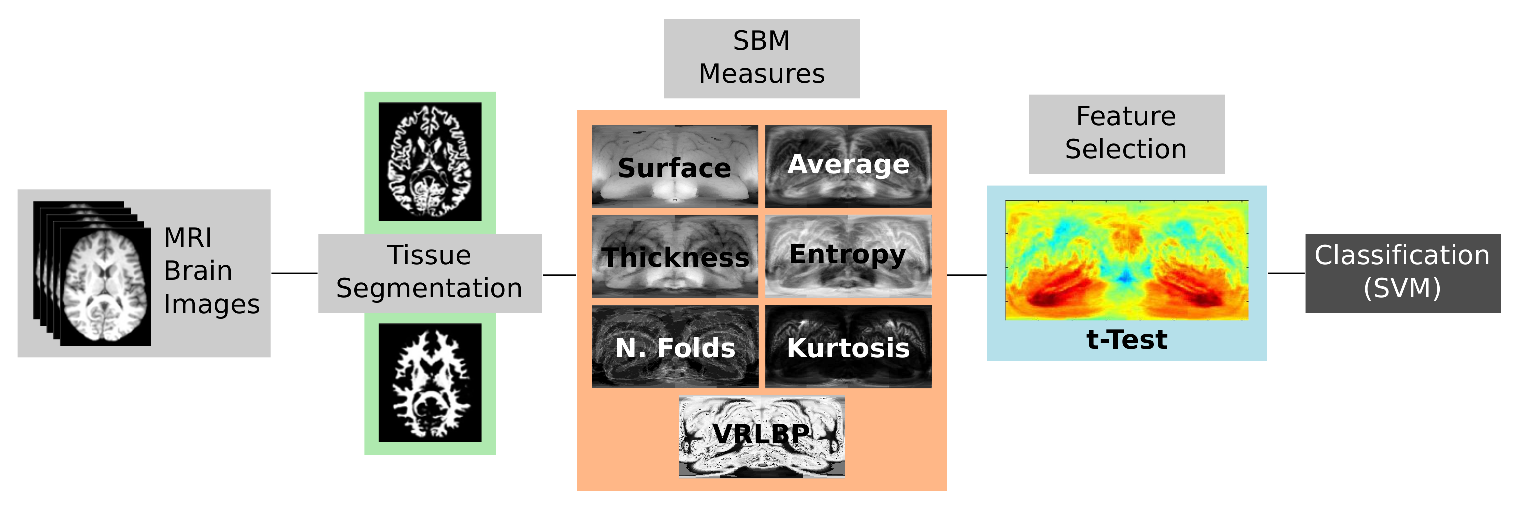
\includegraphics[width=0.8\textwidth]{Graphics/ch6/01-flowdiagram}
	\caption{Flow diagram of the procedure used in the textural analysis of projected MR brain images.}
	\label{fig:flowdiagram}
\end{figure*}

The most relevant extension to the \ac{SBM} was proposed in \cite{Martinez-Murcia2016}. In this work, 

% DONE

The main aim of this work is to provide a new framework that allows the mapping  of a 3D brain image to a two-dimensional space by means of some statistical measures \cite{Martinez-Murcia2015}. The system is based on a conversion from 3D spherical to 2D rectangular coordinates. For each spherical coordinate pair ($\theta,\varphi$), a vector containing all voxels  in the radius is selected, and a number of values are computed, including statistical values (average, entropy, kurtosis) and morphological values (tissue thickness, distance to the central point, number of non-zero blocks). These values conform a two-dimensional image that can be computationally or even visually analysed. In this paper, we proceed using an statistical mask computed using a two-sample $t$-Test, and a SVM classifier. We have achieved performance results that match those obtained with a priori information but using a complete automated procedure, which furthermore reduces the dimensionality of the original images from more than two million voxels to hardly tens of thousands pixels. These maps can be successfully used by itself, but also allow further processing by using them combined and applying some univariate or multivariate algorithms for dimensional reduction. 


In \cite{Martinez-Murcia2015} a new framework called \acf{SBM} was proposed. It was intended to perform feature extraction in MR Brain Images by reducing the whole images to bidimensional maps representing a number a number of statistical and morphological measures. Each pixel in the maps was the result of computing a certain measure on a set of voxels crossed by the mapping vector, a rectilinear vector centred at the \acf{AC} and spanning over all values of azimuth and elevation angles. The bidimensional maps were related to anatomical changes such as brain atrophy or cortical thickness, yielding high performance in differential diagnosis. Furthermore, they provided a significant feature reduction, as well as a visual representation of the underlying information. An extension to the framework using texture and volumetric \acf{LBP} ~\cite{Unay2007} around the mapping vector was proposed in \cite{Martinez-MurciaVRLBP}. 

% Novelty of the work
In this work, we propose a new path tracing algorithm, based on \acfp{HMM}, to enhance the mapping procedure in \ac{SBM} by replacing the mapping vector with curvilinear paths that adapt to the structural information present in MRI. This allows the computation of the feature maps as well as the direct use of the intensity distribution along the path as a characterization of the structural differences in normal or \ac{AD}-affected subjects. Since the Grey Level Co-occurrence Matrix (GLCM), firstly developed by Haralick\cite{Haralick73}, have been used in the characterization of brain in numerous works\cite{martinez2014parametrization,sikio2015mr}, we propose a possible extension intended to characterize the brain texture along each path and its neighbourhood.

\section{Spherical Brain Mapping}
Original \ac{SBM}
\cite{Martinez-Murcia2014225,Martinez-MurciaVRLBP,Martinez-Murcia2015,Martinez-Murcia2016}

The technique proposed to perform the mapping of the 3D brain images to a 2D map using spherical coordinates -from now on \acf{SBM}-  is based on the use of spherical coordinates in the brain. A base  point is set in the central voxel of the MRI image, and a mapping vector $\mathbf{v}_{\theta,\varphi}$ of length $N$ is defined for each inclination ($\theta$) and azimuth ($\varphi$) angles in the range $0^{\circ}<\theta<180^{\circ}$ and $0^{\circ}<\varphi<360^{\circ}$ (see Figure~\ref{fig:brainmapping}). Therefore, we will define the sampled set $V_{\theta,\varphi}$, a set that contains $P$ voxels crossed by the sampling vector $\mathbf{v}_{\theta,\varphi}$.
For each set $\mathbf{v}_{\theta,\varphi}$, a mapping value $v$ is computed from the sampled voxels $V_{\theta,\varphi}$, depending on the  measure used. In this section, six basic measures are proposed:

\begin{figure}[htp]
	\centering
	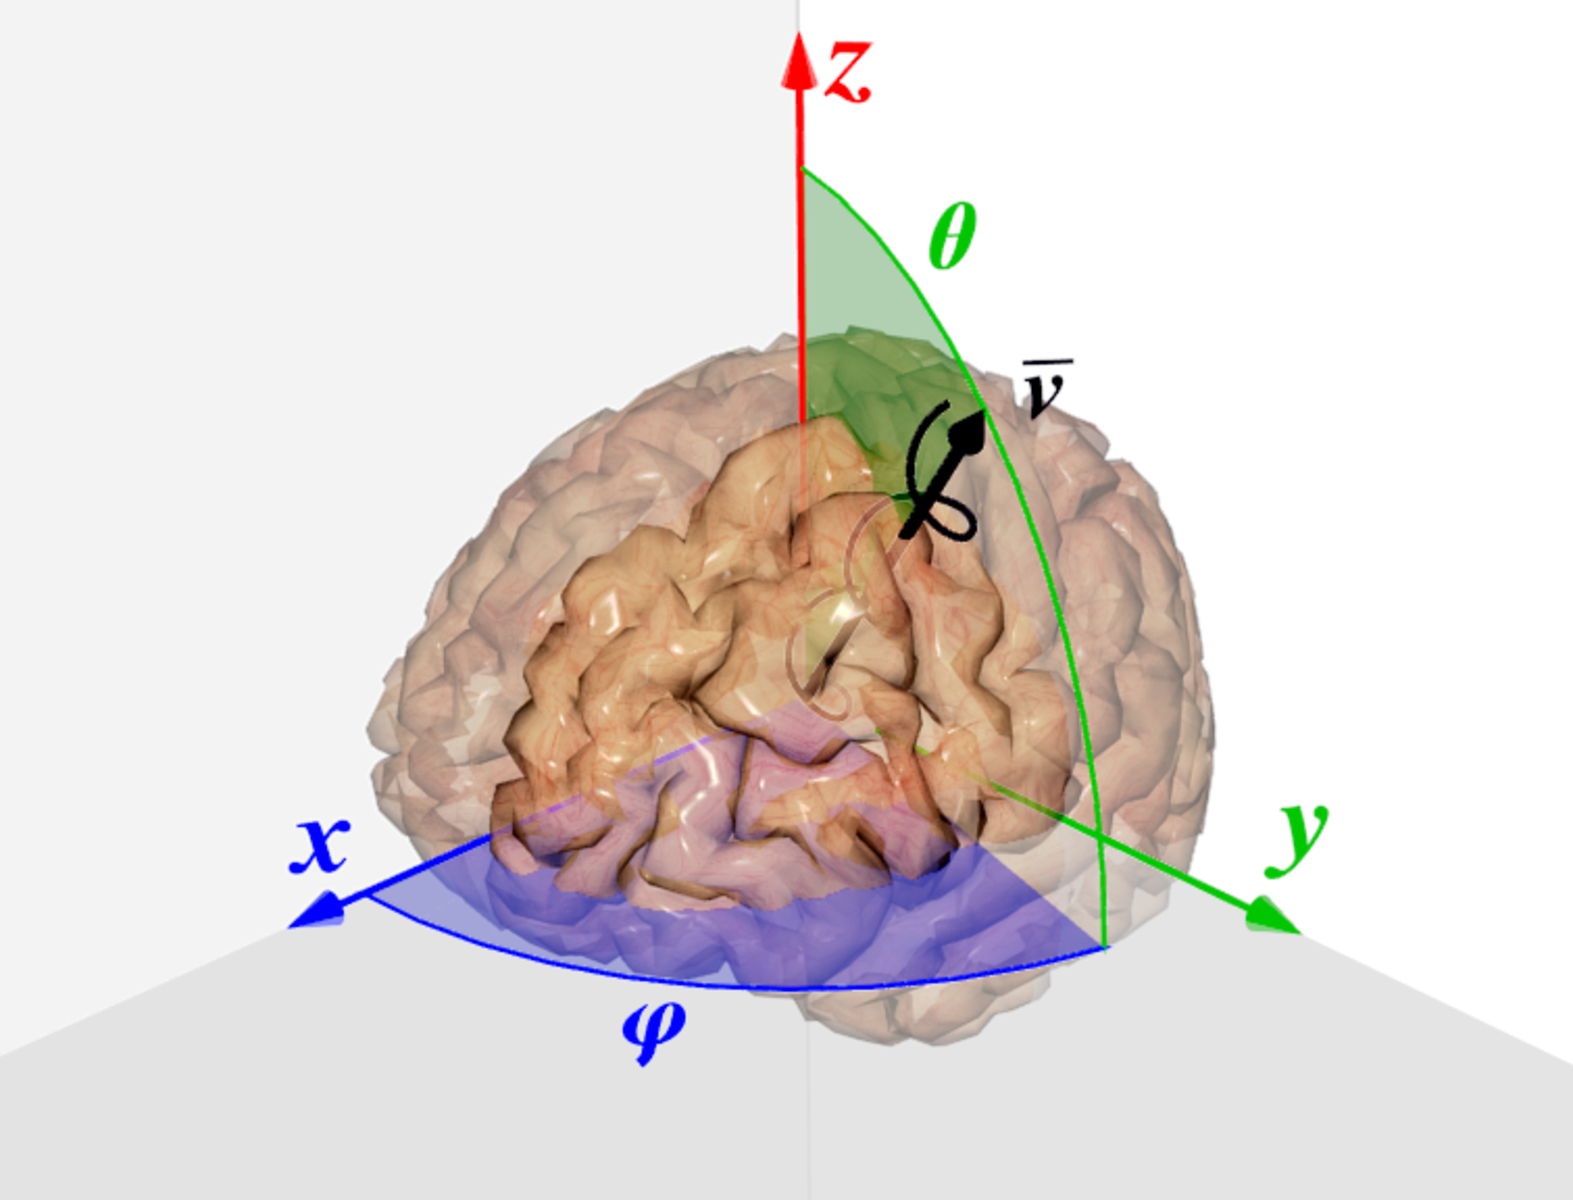
\includegraphics[width=0.8\columnwidth]{Graphics/ch6/02-projection}
	\caption{Illustration of the computation of the mapping vector $\mathbf{v}_{\theta,\varphi}$, the angles $\theta$ and $\varphi$ and the $r$-neighbourhood of $\mathbf{v}$ (see Section~\ref{sec:vrlbp}).}
	\label{fig:brainmapping}
\end{figure}

\begin{itemize}
	\item A basic \underline{brain surface} approach, that accounts for the distance between the central voxel and the last tissue voxel in $V_{\theta,\varphi}$ that is greater than a threshold $I_{th}$. This might allow our system to observe structural degeneration and tissue loss in the surface of the tissue. 
	\begin{equation}\label{eq:surface}
	v_{surf}= \argmax_i \lbrace V_{\theta,\varphi}(i)>I_{th}\rbrace \quad \forall i=1,\dots P
	\end{equation}  
	
	\item Another parameter used is \underline{thickness} of the tissue. This can be useful when measuring the thickness of segmented Gray Matter or White Matter MR images. It is defined as the distance between the last and first elements in $V_{\theta,\varphi}$
	with an intensity greater than a threshold $I_{th}$ (typically 0): 
	\begin{equation}\label{eq:thickness}
	v_{thick}=\argmax_i \lbrace V_{\theta,\varphi}(i)>I_{th}\rbrace- \argmin_i \lbrace V_{\theta,\varphi}(i)>I_{th}\rbrace
	\quad \forall i=1,\dots P
	\end{equation}  
	
	\item The \underline{number of folds} represents the number of overlapping segments of tissue in the set $V_{\theta,\varphi}$. It is computed by thresholding $V_{\theta,\varphi}$ using the value $I_{th}$ and counting the number of resulting connected subsets. Let $A_{\theta,\varphi}$ be the set that contains all the indices of the voxels in $V_{\theta,\varphi}$ with an intensity greater than $I_{th}$:
	\begin{equation}
	A_{\theta,\varphi} = \lbrace i \; / \: V_{\theta,\varphi}(i)>I_{th} \rbrace
	\end{equation}
	where $A_{\theta,\varphi} \in \mathbb{N}$. Let us divide $A_{\theta,\varphi}$ in $J$ disjoint connected subsets so that:
	\begin{equation}
	A_{\theta,\varphi} = A_{\theta,\varphi}^1 \cup A_{\theta,\varphi}^2 \cup \dots \cup A_{\theta,\varphi}^J \quad \text{so that} \quad A_{\theta,\varphi}^i \cap A_{\theta,\varphi}^j = \emptyset \quad \forall i,j
	\end{equation}
	Therefore, our $v_{nf}=J$, the number of disjoint connected subsets in $A_{\theta,\varphi}$.
	
	\item An \underline{average} approach, where the average of all the intensity values in the set $V_{\theta,\varphi}$ is computed as: 
	\begin{equation}\label{eq:mean}
	v_{av}=\frac{1}{N}\sum_i V_{\theta,\varphi}(i) \quad \forall i=1,\dots P
	\end{equation}  
	
	\item The \underline{entropy} assumes that the set $V_{\theta,\varphi}$ is a probability mass vector (probability of belonging to a certain tissue, normalized) and computes $v$ as:
	\begin{equation}
	v_{ent}=\sum_i V_{\theta,\varphi}(i)*\log(V_{\theta,\varphi}(i)) \quad \forall i \in \arg_i\lbrace V_{\theta,\varphi}(i)>0\rbrace
	\end{equation}
	
	\item The uncorrected \underline{kurtosis}, also known as fourth standardized moment, of the set $V_{\theta,\varphi}$ in which $v$ is calculated using:
	\begin{equation}
	v_{kurt}= \frac{\frac{1}{N}\sum_i\left(V_{\theta,\varphi}(i)-\bar{V}_{\theta,\varphi}(i)\right)^4}{\left(\frac{1}{N}\sum_i\left(V_{\theta,\varphi(i)}-\bar{V}_{\theta,\varphi}(i)\right)^2\right)^2} \quad \forall i=1,\dots P
	\end{equation}
	where $\bar{V}_{\theta,\varphi}$ is the average of all voxels in $V_{\theta,\varphi}$ (same value as $v_{av}$, described in Eq.~\ref{eq:mean}). 
	
\end{itemize}

The resulting \ac{GM} and \ac{WM} maps are depicted in Figure~\ref{fig:masksGM}. 

\begin{figure*}[htp]
	\centering
	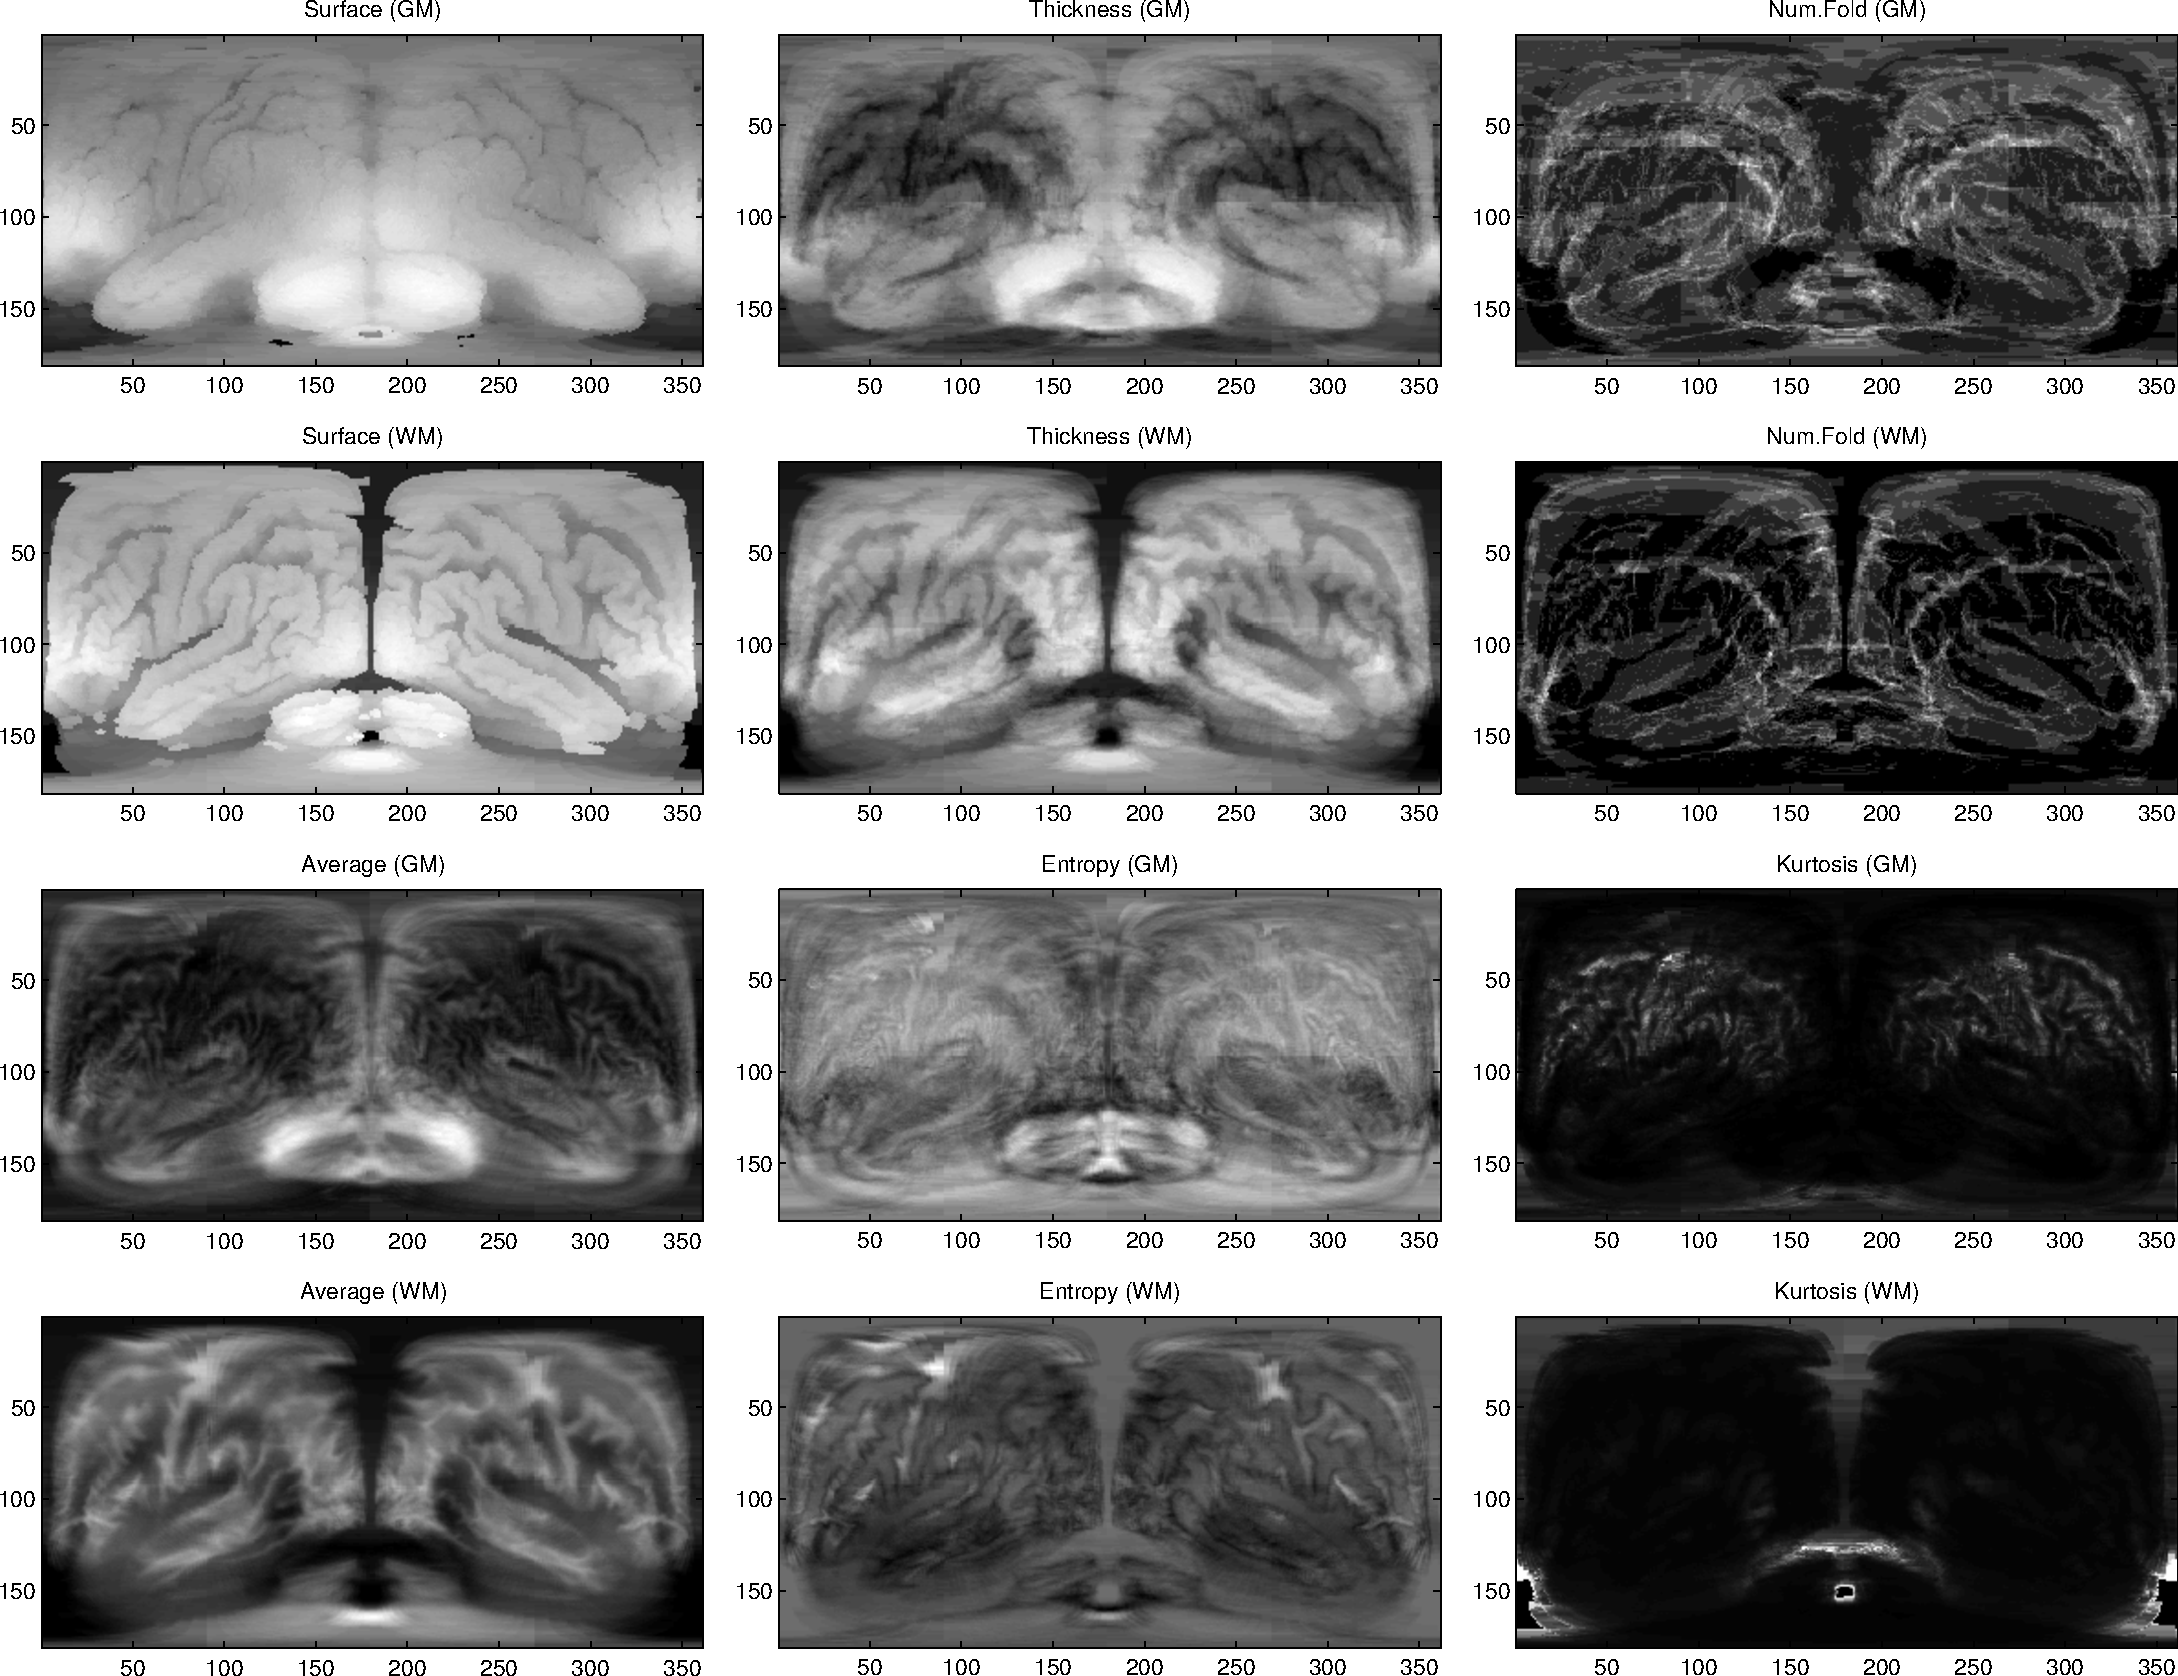
\includegraphics[width=1\textwidth]{Graphics/ch6/03-projections}
	
	\caption{Resulting \ac{GM} and \ac{WM} maps of the same control subject using the six proposed measures: Surface, Thickness, Number of Folds, Average, Entropy and Kurtosis.}
	\label{fig:masksGM}
\end{figure*}

The resulting maps will contain the value $v$ mapped in each direction $(\theta,\varphi)$. As the inclination angle $\theta$ ranges from $0^{\circ}$ to $180^{\circ}$ and the azimuth $\varphi$ from $0^{\circ}$ to $360^{\circ}$, the resulting maps will have a size of $181\times361$, where each pixel is the $v$ value for each direction. The whole algorithm can be downloaded at \url{http://wdb.ugr.es/~fjesusmartinez/portfolio/sbm/}.

This methodology defines the sampling set as the voxels that are crossed by the sampling vector $\mathbf{v}_{\theta,\varphi}$. When projecting a structure as complex as the brain, this implies a loss of contextual information of both the neighbourhood and the layers crossed by $\mathbf{v}_{\theta,\varphi}$. Two approaches have been suggested to overcome this problem: the first one extends the system by dividing the sampling set $V_{\theta,\varphi}$ in $n$ equal parts in a so-called ``Layered approach'', and the second one uses a helical sampling and Local Binary Patterns (LBP) to map the neighbourhood of the sampling vector and characterize the texture of the area.


\subsection{Layered Extension}\label{sec:layered}
The first strategy used to improve the descriptive abilities of the mappings is the Layered Extension. In this approach, the sampled voxels set $V_{\theta,\varphi}$ can be divided in $n$ equal subsets, using each one to project one section -or layer- of the brain. If, for example, we use $n=4$, $4$ subsets containing the same number of voxels  will be derived from $V_{\theta,\varphi}$, and therefore $4$ different maps  will be depicted, from the closest to the centre to the farthest. This layered approach reveals  the different anatomical structures found in the brain at different depths, potentially revealing a more detailed distribution the features  of the mappings . These layered maps and their performance will be discussed later.

\section{Volumetric Radial LBP}\label{sec:vrlbp}
In a second attempt to overcome the loss of per layer information, we have expanded the influence of $\mathbf{v}_{\theta,\varphi}$ to its $r$-neighbourhood. This has been done by defining a $v$ measure that describes not only the features of the voxels crossed by $\mathbf{v}_{\theta,\varphi}$, but the texture of its neighbourhood using a Volumetric Radial Volumetric Radial Local Binary Pattern (VRLBP) descriptor.

Local Binary Patterns (LBP) were first introduced in \cite{Ojala1996} to describe the texture of an image with application to face recognition. Later, in \cite{Zhao2007}, the technique was extended to a Volume LBP (VLBP), defining a 3D texture in a local neighbourhood by using a cylinder oriented in one direction and whose radius define the neighbourhood used to compute the LBP descriptor. 

In the VRLBP, the sampling method devised in \cite{Zhao2007} has been updated to follow helical coordinates around the mapping vector $\mathbf{v}_{\theta,\varphi}$ (see helix around $\mathbf{v}_{\theta,\varphi}$ in Figure~\ref{fig:brainmapping}). Formally, we note $V_{\theta,\varphi}^{P,r}$ the set of $P$ sampled voxels of the image $I$ in the $r$-neighbourhood of $\mathbf{v}_{\theta,\varphi}$ taken by helical sampling:

\begin{equation}
V_{\theta,\varphi}^{P,r}=\lbrace I(g_{\theta,\varphi}^{0,r}), I(g_{\theta,\varphi}^{1,r}), I(g_{\theta,\varphi}^{2,r}), \dots I(g_{\theta,\varphi}^{P-1,r})\rbrace
\end{equation} 
where the coordinates $g_{\theta,\varphi}^{p,r}$ of each voxel are computed in the direction of $\mathbf{v}_{\theta,\varphi}$ by: 
\begin{equation}
\label{ec:helical_coordinates}
g_{\theta,\varphi}^{p,r}=\begin{cases}
x_{\theta,\varphi}^{p,r}=p\sin(\varphi)\cos(\theta)-r\sin(2\pi n\frac{p}{P})\\
y_{\theta,\varphi}^{p,r}=p\sin(\varphi)\sin(\theta)+r\cos(2\pi n\frac{p}{P})\\
z_{\theta,\varphi}^{p,r}=p\cos(\varphi) 
\end{cases} \quad p=\{0,...,P-1\}, P \in \mathbb{N}
\end{equation}
being $n$ the number of loops in the helix. Following \cite{Zhao2007}, voxels that do not fall exactly at the coordinates computed in the equations \ref{ec:helical_coordinates} are estimated by interpolation.

Let us assume, without lost of generality, that $P$ and $r$ are fixed. This way, set of sampled voxels $V_{\theta,\varphi}^{P,r}$ becomes $V_{\theta,\varphi}$, which matches the definition of Section~\ref{sec:mapping}. Following this notation, the value $v$ for this VRLBP approach is computed using: 

\begin{equation}
v_{VRLBP} = \sum_{i} s(V_{\theta,\varphi}(i)-V_{\theta,\varphi}(0))\cdot 2^{i} \quad \forall i=1,\dots P
\end{equation}
where $s(x)$ is the sign function, defined as: 
\begin{equation} % He simplificado la formula usando "cases"
s(x) = 
\begin{cases}
1      &  x \geq 0 \\
0      &  x < 0
\end{cases}
\end{equation}
This approach provides textural information about all brain structures in a certain direction, as it can be seen in Figure~\ref{fig:vrlbp}. 

\begin{figure*}[htp]
	\centering
	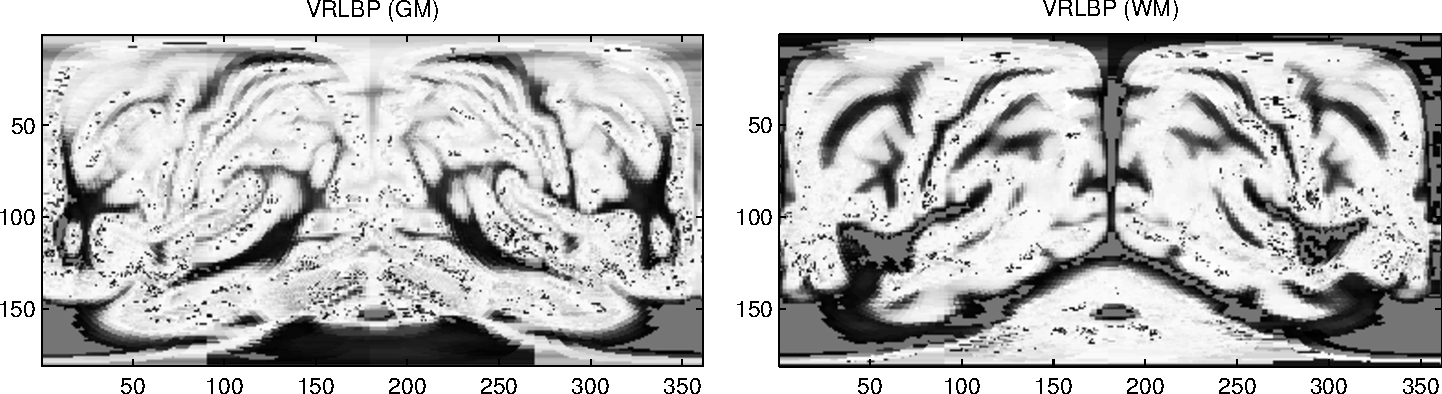
\includegraphics[width=\textwidth]{Graphics/ch6/04-vrlbp}
	\caption{An example of the VRLBP projection for \ac{GM} and \ac{WM} Tissues. }
	\label{fig:vrlbp}
\end{figure*}


\lstset{language=python} 
\begin{lstlisting}
	def foo():
		hola amigo
		print('amigo')
	
	eh = foo("amigo")
	
	string title = "This is a Unicode $\pi$ in the sky"
	/*
	Defined as $\pi=\lim_{n\to\infty}\frac{P_n}{d}$ where $P$ is the perimeter
	of an $n$-sided regular polygon circumscribing a
	circle of diameter $d$.
	*/
	const double pi = 3.1415926535
\end{lstlisting}

\section{Path via Hidden Markov Models}
We have already talked about the limitations of the rectilinear mapping vector used in \cite{Martinez-Murcia2015} and \cite{Martinez-MurciaVRLBP}. Therefore, it would be desirable to define new mapping paths that use all the available intensity and spatial information in MRI images. This way, the resulting sets of selected voxels (and the resulting maps) would contain information about both the intensities and structure.

% Algoritmo base de extracción de puntos
To define the paths, we can define 3D Biomedical Images as a tuple containing spatial information in the image range ($\mathbf{x} \in \mathbb{I}$, where $\mathbb{I}\subset \mathbb{R}^3$) as well as intensity information ($I(\mathbf{x}) \in \mathbb{R}$). There exist a number of possibilities in the interpretation of intensity data on the images, from plain intensity values to a sampling of the underlying tissue density (and thus, an estimation of the probability of finding tissue in each position). 

Following our \ac{SBM} approach, in which some radia are used to extract relevant statistical features from these images, we formulate a 3D path tracing algorithm suitable for extraction of curvilinear structures from 3D biomedical images, and directly linked to each direction $(\varphi,\theta)$ as in the original work. Our objective is to make these paths as representative of the underlying intensity distribution as possible. To do so, we must use both intensity and spatial information to construct maximum intensity-similarity paths oriented in the given direction. 

Let us note a 3D path in a certain direction $(\varphi,\theta)$ as a Markov Model\cite{Chen2008}: 
\begin{equation}
\mathbf{X} = \{\mathbf{x}_0, \mathbf{x}_1, \mathbf{x}_2, \dots \mathbf{x}_N\}
\end{equation}
Therefore, our optimum path would be the one that maximizes the probability of the path:
\begin{equation}\label{eq:optimalPath}
\mathbf{X}_{opt} = \argmax_\mathbf{X} \{P(\mathbf{X})\}
\end{equation}
or, similarly, the probability of all the nodes:
\begin{equation}\label{eq:probPath}
P(\mathbf{X}) = P(\mathbf{x}_0, \mathbf{x}_1, \mathbf{x}_2, \dots \mathbf{x}_N)
\end{equation}
where $\mathbf{x}_0$ is the node located at the AC and $\mathbf{x}_N$ is the theoretical projection of the current direction $(\varphi,\theta)$ in the limits of the image $\mathbb{I}$. Setting $\mathbf{x}_0$ at the AC is not a random choice; it is a convention when using the \ac{MNI} coordinates\cite{Evans1993} and furthermore, since it is a point that shares connectivity with both hemispheres, the resulting paths will be optimal, covering most of the brain. We can assume a first-order \acf{HMM} for the tracing of the path, and the $i$-th node will be computed as:
\begin{equation}
P(\mathbf{x}_i | \mathbf{x}_{i-1}, \mathbf{x}_{i-2}, \dots \mathbf{x}_0) \approx P(\mathbf{x}_i|\mathbf{x}_{i-1})
\end{equation}
and with this assumption, (\ref{eq:probPath}) becomes:
\begin{equation}
P(\mathbf{X}) = P(\mathbf{x}_0, \mathbf{x}_1, \dots \mathbf{x}_N) = \prod_{i=1}^{N} P(\mathbf{x}_i|\mathbf{x}_{i-1})
\end{equation} 

In our case, we will assume that the hidden state of each node will be its intensity $I(\mathbf{x}_i)$. Let $\mathbf{I} = \{I(\mathbf{x}_0), I(\mathbf{x}_1), \dots I(\mathbf{x}_N)\}$ be the vector of the intensities in each node. With the introduction of these factors, our optimal path defined in (\ref{eq:optimalPath}) can be view as:
\begin{align}
\mathbf{X}_{opt} & = \argmax_\mathbf{X} \{P(\mathbf{X}|\mathbf{I})\}\\
P(\mathbf{X}|\mathbf{I}) & = P(\mathbf{x}_0, \dots x_N| I(\mathbf{x}_0), \dots I(\mathbf{x}_N))\\
& = \frac{P(I(\mathbf{x}_0), \dots I(\mathbf{x}_N)|\mathbf{x}_0, \dots x_N)\cdot P(\mathbf{x}_0, \dots x_N)}{P(I(\mathbf{x}_0), \dots I(\mathbf{x}_N))}\label{eq:final}
\end{align}
where:
\begin{equation}\label{eq:intP}
P(I(\mathbf{x}_0), \dots I(\mathbf{x}_N)|\mathbf{x}_0, \dots x_N)  = \prod_{i=1}^{N} P (I(\mathbf{x}_i)|\mathbf{x}_i)
\end{equation}
and $P(I(\mathbf{x}_0), \dots I(\mathbf{x}_N))$ is the \textit{a priori} probability of the intensities in the path. We can assume, without lack of generality, that this term is constant along the path, and therefore, it plays no part in the optimization process.

For computational purposes, we will compute all the needed probabilities on a set of candidates $\mathbf{X}_c = \{\mathbf{x}_{c,1}, \mathbf{x}_{c,2}, \dots \mathbf{x}_{c,M} \}$ defined by $\mathbf{x}_{i-1}$. This candidates are contained inside the $L^2$-norm support ball $B_{2,r}(\mathbf{x}-\mathbf{x}_{i-1})$ of radius $r$ centred in $\mathbf{x}_{i-1}$.

To estimate the individual probabilities needed for (\ref{eq:intP}) $P (I(\mathbf{x}_i)|\mathbf{x}_i)$, we can assume a normal distribution of intensities of the candidates with mean $I(\mathbf{x}_{i-1})$ and variance $\sigma_c^2$ the variance of the intensities of the candidate set. By assuming this, the probability of a certain intensity in the candidate node $\mathbf{x}_i$ increases as the intensity becomes more similar to the intensity of $\mathbf{x}_{i-1}$. Therefore, the assumption supports the tracing of minimal intensity difference paths. The probability of the intensity of a candidate $\mathbf{x}_i$ will be: 
\begin{equation}\label{eq:intensity}
P(I(\mathbf{x}_i)|\mathbf{x}_i) =\frac{1}{\sqrt{2\pi \sigma_c^2}}\exp\left(-\frac{(I(\mathbf{x}_i)-I(\mathbf{x}_{i-1}))^2}{2\sigma_c^2}\right)
\end{equation}

The last term $P(\mathbf{x}_0, \dots \mathbf{x}_N)$ to be defined in (\ref{eq:final}) is directly related to the \ac{SBM} framework defined before, as it will depend on the radial direction $(\varphi, \theta)$ that we want to ``force'' in the path. To define this term, we will define an attractor located in the position $\mathbf{x}_N$ (the projection of the current direction $(\varphi,\theta)$ in the limits of the image $\mathbb{I}$). We assume that this attractor defines the conditionality, that is, that it affects the transition probability between states by means of an isotropic Gaussian radial basis function (RBF), as defined in (\ref{eq:rbf}). This definition helps the attractor to lightly condition the direction of the path at first, and more strongly as the path approaches the cortex, leading to a better representation of the underlying structure. 
\begin{align}\label{eq:rbf}
&P(\mathbf{x}_0, \dots \mathbf{x}_N) = P(\mathbf{x}_i|\mathbf{x}_N)  \\&= \frac{1}{\sqrt{(2\pi)^d|\Sigma|}} \exp\left(-\frac{1}{2}(\mathbf{x}_i-\mathbf{x}_N)\Sigma^{-1}(\mathbf{x}_i-\mathbf{x}_N)\right) 
\end{align}
where $\Sigma$ is the covariance matrix of the given distribution. As we will consider only isotropic gaussian kernel, the matrix can be considered as a $3\times3$ diagonal matrix whose diagonal elements are a scalar value $\sigma^2$, which we set in each iteration to the euclidean distance between $\mathbf{x}_i$ and $\mathbf{x}_N$. 

\subsubsection{Step Size}
In this algorithm, instead of using a fixed step size, we evaluate each candidate point $\mathbf{x} \in B_{2,r}(\mathbf{x}-\mathbf{x}_i)$, and thus, the only parameter to regulate is the radius of the L2-norm support ball $r$. As a trade-off between computational issues and definition of the defined path, we will use a value of $r=3$ voxels, which gives approximately $200$ candidate points in each iteration. 

\subsubsection{Stop Condition}
Although the paths could be defined until they reach the last point $\mathbf{x}_N$ (remember, the projection of the general direction onto the limits of $\mathbb{I}$), our interest is to model the paths inside the brain, and therefore we establish a stop condition using an intensity threshold. This threshold is computed using the entropic thresholding, as defined in \cite{Yen1995}. Let $G_m \equiv \{I_0, I_1, ... I_m\} $ denote the set of intensity levels of the whole image. We can compute a histogram to obtain the observed frequencies $f_{I_i}$, and thus, the observed probability of the different Grey levels $p_{i} = f_{I_i}/N$, where $N$ is the number of voxels in our image $\mathbb{I}$.

For a given intensity threshold $I_{th}=I_s$, if $\sum_{i=0}^{s-1}p_i$ is larger than zero and smaller than 1, the following distributions can be derived from this distribution after normalization:
\begin{align}
& A \equiv \left\{\frac{p_0}{P(I_{s})}, \frac{p_1}{P(I_{s})}, \dots, \frac{p_{s-1}}{P(I_{s})} \right\}\\
& B \equiv \left\{\frac{p_{s}}{1-P(I_{s})}, \frac{p_{s+1}}{1-P(I_{s})}, \dots, \frac{p_m}{1-P(I_{s})} \right\}
\end{align}
where $P(I_s) = \sum_{i}^{s}p_{I_i}$ is the cumulative density function for the $s$-th Grey level. Therefore, we choose the threshold so that the total amount of information provided by $A$ and $B$ (foreground and background of the image) is maximized. The total information provided by the $s$-th Grey level is: 
\begin{align}
TE(s) & = E_A(s) + E_B(s) \\
& = -\sum_{i=0}^{s-1}\left(\frac{p_i}{P(I_s)}\right)\log\left(\frac{p_i}{P(I_s)}\right) \\
& - \sum_{i=s}^{m-1}\left(\frac{p_i}{1-P(I_s)}\right)\log\left(\frac{p_i}{1-P(I_s)}\right)
\end{align}

A summary of our \ac{HMM}-based path tracing method is shown in Algorithm~\ref{alg:hmmPath}. To illustrate the effect of the algorithm on a real example, Fig.~\ref{fig:cuts} depicts the resulting set of paths computed over the standard MRI DARTEL template. 

\begin{algorithm*}
	\SetKwData{CandInt}{candInt}
	\SetKwData{PathList}{pathList}
	\SetKwInOut{Input}{input}
	\SetKwInOut{Output}{output}
	\Input{MRI Brain Image $I$ of size $U\times V\times W$, $\mathbf{x}_0$}
	\Output{List of nodes in the optimum path $\mathbf{X}_{opt}$}
	\BlankLine
	Compute the $I_{th} = I_s$ where $s$ maximizes $TE(s)$\;
	Set $\mathbf{x}_0$ to the AC\;
	%\For{$\varphi\leftarrow -180$ \KwTo $180$}{
	%	\For{$\theta\leftarrow -90$ \KwTo $90$}{
	Compute the attractor position $\mathbf{x}_N$ in the direction $(\varphi, \theta)$\;
	$\mathbf{x}_i \leftarrow \mathbf{x}_0$\;
	\While{$(i<\text{IterLimit})$ \& $(I(\mathbf{x}_i)>I_{th})$ \& ($\mathbf{x}_i \in \mathbb{I}$)}{
		Get the node candidates $\mathbf{X}_c = \{\mathbf{x}_{c,1}, \mathbf{x}_{c,2}, \dots \mathbf{x}_{c,M}\}$ where $\mathbf{x}_{c,m} \in B_{2,r}(\mathbf{x}_{c,m}-\mathbf{x}_i)$\;
		Get the intensities of the candidates $I(\mathbf{x}_c) \quad \forall \mathbf{x}_c \in \mathbf{X}_c$\;
		\textbf{foreach} $\mathbf{x}_c \in \mathbf{X}_c${
			compute $P(\mathbf{x}_c|\mathbf{x}_N)$ and $P(I(\mathbf{x}_c)|\mathbf{x}_i)$  \;
		}
		$\mathbf{x}_{i+1} = \argmax_{\mathbf{x}_c} [P(I(\mathbf{x}_c)|\mathbf{x}_i)\cdot P(\mathbf{x}_c|\mathbf{x}_N)]$\;
		$i=i+1$\;
	}
	$\mathbf{X}_{opt}\leftarrow \{\mathbf{x}_0, \mathbf{x}_1, \dots \mathbf{x}_N\}$\; 
	%	}
	%}
	
	\caption[\acs{HMM}-based Path Creation]{\ac{HMM}-based Path Creation}\label{alg:hmmPath}
\end{algorithm*}\DecMargin{1em}


\begin{figure}
	\begin{center}
		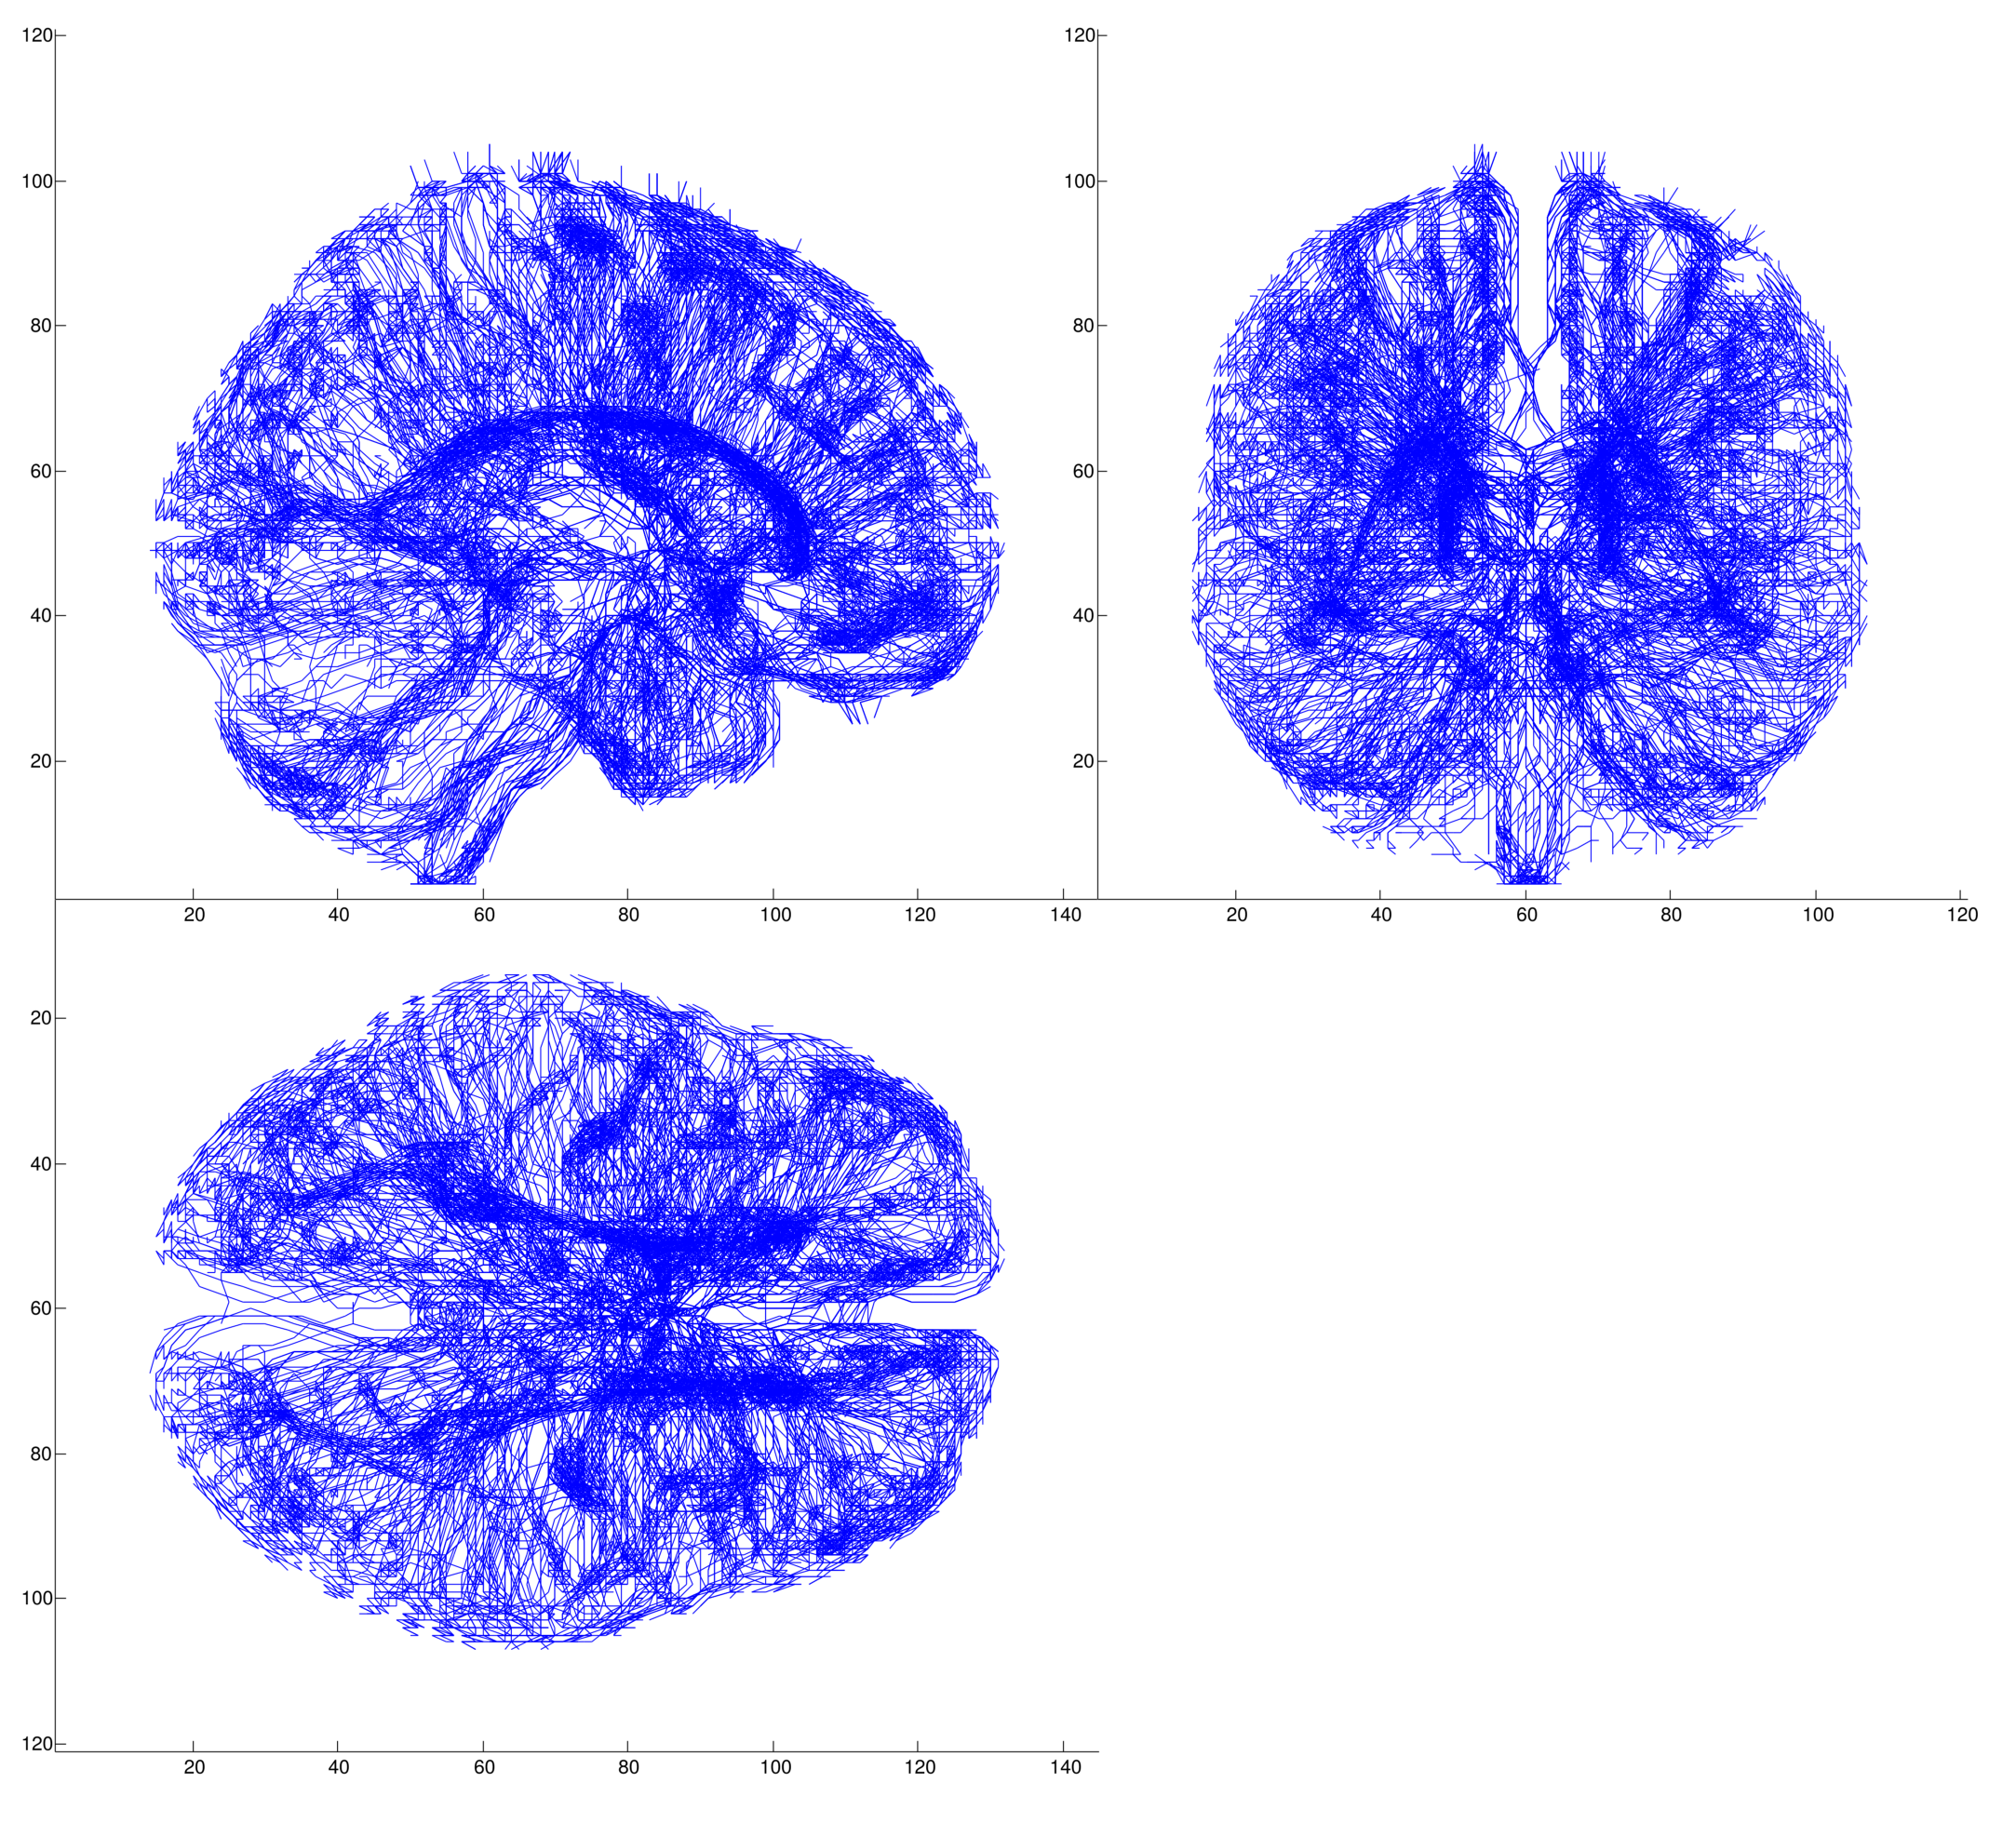
\includegraphics[width=2in]{Graphics/ch6/cuts}
		\caption[Set of \acs{HMM} based paths over the MRI DARTEL template.]{Set of \ac{HMM} based paths over the MRI DARTEL template.}
		\label{fig:cuts}
	\end{center}
\end{figure}


% Con o sin suavizado
\subsection{Radial Texture Features}\label{sec:rtextfeat}
The paths extracted with the aforementioned algorithm present a meaningful representation of the structure of the intensity levels (and therefore, the tissue density) of the MRI brain images. At this point, one might consider using the intensity values located in those radia as features, and try to characterize each radius' discrimination ability by means of these intensities. 

Conversely, the strategy proposed in \cite{Martinez-MurciaVRLBP}, which uses Local Binary Pattern (LBP) descriptors in the helical neighbourhood of a rectilinear mapping vector, might be a complementary approach. Due to the \ac{HMM} paths topology, the helical sampling becomes difficult to compute and not even useful, therefore we propose a modification of the Grey Level Co-occurrence Matrix (GLCM) along the paths. 

The GLCM, proposed by Haralick\cite{Haralick73}, is one of the most widely used methods in texture characterization, and it has been successfully applied to medical imaging in the past\cite{kovalev2001three,martinez2014parametrization}. It works by storing the number of voxel-wise correspondences between $K$ grey levels with a certain position offset $\Delta$ on a  $K\times K$ matrix ($C_{\Delta}$) along all the image. 

Our modification will compute a node-wise GLC matrix, in which the number of grey-level transitions between adjacent nodes, noted as $\mathbf{x}_i$ and $\mathbf{x}_{i+1}$, is stored along the whole path $\mathbf{X} = \{\mathbf{x}_0, \mathbf{x}_1 \dots \mathbf{x}_N\}$. Mathematically, the computation of the GLCM in each point in the path will be: 
\begin{equation}\label{eq:glcm}
C_{\Delta_i}(j,k) = \sum_{i=0}^{N-1}
\begin{cases}
1 & I(\mathbf{x}_i) = j, I(\mathbf{x}_{i+1})=k\\
0 & otherwise
\end{cases}
\end{equation}
where the offset is different for each pair of nodes $\Delta_i=\mathbf{x}_{i+1}-\mathbf{x}_i$. 

The definition provided in (\ref{eq:glcm}) is intended for computing the values in each node. However, we can generalize this construction to include not only the nodes, but the intensity information around each node in the computation, which could potentially lead to more significant texture features. Let us note a set containing all the voxels in the closed neighbourhood of $\mathbf{x}_i$ as $X_i$. Therefore, (\ref{eq:glcm}) can be generalized for any voxel $\mathbf{x} \in X_i$ as:
\begin{equation}\label{eq:glcmGen}
C(j,k) = \sum_{i=0}^{N-1} \sum_{\mathbf{x} \in X_i}
\begin{cases}
1 & I(\mathbf{x}) = j, I(\mathbf{x}+\Delta_i)=k\\
0 & otherwise
\end{cases}
\end{equation}

From the GLCM, a variety of texture descriptors, or features, can be extracted. In this work we will use ten texture features proposed in the original Haralick's article\cite{Haralick73} as well as in Refs~\cite{soh1999texture} and \cite{clausi2002analysis}: Contrast\cite{Haralick73}, Correlation\cite{Haralick73}, Dissimilarity\cite{soh1999texture}, Energy\cite{Haralick73}, Entropy\cite{soh1999texture}, Homogeneity\cite{Haralick73}, Difference Variance\cite{Haralick73} (D. Variance), Difference Entropy\cite{Haralick73} (D. Entropy), Inverse Difference Normalized\cite{clausi2002analysis} (IDN) and Inverse Difference Moment Normalized\cite{clausi2002analysis} (IDMN). The mathematical expressions for these features are presented in Equations~\ref{eq:contrast} to \ref{eq:idmn}.

\begin{align}\label{eq:contrast}
\text{Contrast} &= \textstyle\sum_j\sum_k\{(j-k)^2C(j,k)\}\\
%\sum_{n=0}^{N_g-1}n^2 \left\{\sum_{j=1}^{N_g}\sum_{k=1}^{N_g}C(j,k)\right\}, |j-k|=n\\
\text{Correlation} &= \textstyle\frac{\sum_j\sum_k(j-\mu_j)(k-\mu_k)C(j,k)}{(\sigma_j\sigma_k)}\\ % matlab
\text{Dissimilarity} & = \textstyle\sum_j\sum_k\{|j-k|C(j,k)\}\\
\text{Energy} &= \textstyle\sum_j\sum_k C(j,k)^2\\
\text{Entropy} &= - \textstyle\sum_j\sum_kC(j,k)\log(C(j,k))\\
\text{Homogeneity} &= \textstyle\sum_j\sum_k \frac{C(j,k)}{1+|j-k|}\\ % matlab
\text{D. Variance} &= \textstyle\sum_{j=0}^{N_g-1}j^2 p_{x-y}(j)\\
\text{D. Entropy} &= -\textstyle\sum_{j=0}^{N_g-1} p_{x-y}(j)\log\{p_{x-y}(j)\}\\
\text{IDN} &= \textstyle\sum_j\sum_k \frac{C(j,k)}{1+|j-k|/N}\\ \label{eq:idmn}
\text{IDMN} &= \textstyle\sum_j\sum_k \frac{C(j,k)}{1+(j-k)^2/N^2}
%\text{SSVAR} &= \textstyle\sum_j\sum_k(j-\mu)^2C(j,k)\\
%\text{CLP} &= \textstyle\sum_j\sum_k(j-\mu)^2C(j,k)\\
%\text{SAV} &= \textstyle\sum_{j=2}^{2N_g}jp_{x+y}(j)\\
%\text{SVAR} &= \textstyle\sum_{j=2}^{2N_g}(j-f_8)^2p_{x+y}(j)\\
%\text{SENT} &= - \textstyle\sum_{j=2}^{2N_g}p_{x+y}(j)\log\{p_{x+y}(j)\}\\
%\text{HOMOP} &= \textstyle\sum_j\sum_k\frac{C(j,k)}{1+(j-k)^2}\\
%\text{jMC1} &= \frac{ENT-HXY1}{\max(HX,HY)}\\
%\text{jMC2} &= (1-\exp\left\{-2(HXY2-HXY)\right\})^\frac{1}{3}\\
\end{align}


\section{Results}

\subsection{Experimental settings and validation}\label{sec:experimental}
In this work, have considered a binary classification problem: AD vs. NC, where we have evaluate separately each type of mapping. First, in Section~\ref{sec:significance}, we will analyse our maps by means of the $t$ statistic, where the areas of higher statistical significance (AD vs NC) will be highlighted. To better interpret the results, an anatomical reference is provided.

Second, we have perform a classification analysis using feature selection by means of $t$-Test, then training and testing a linear SVM classifier. The method has been validated using
stratified 10-fold cross-validation, as recommended in \cite{Kohavi1995a}.  This procedure consists on randomly partition the whole datasets into 10 subsets that contains the same proportion of individual of both classes as the whole database. Then, one subset is used for testing and the remaining 9 are used for training. This is repeated for each of the subsets as training sets. Finally, the whole cross-validation strategy will be repeated 10 times to avoid the possible bias and random effects of the partitions, and obtain the average and standard deviation of the performance values. 

Values of accuracy (acc), sensitivity (sens) and specificity (spec) along with their standard deviation  will be employed to evaluate the performance of the different mappings. Selection of parameter $C$ of the SVM classifier (as implemented in \texttt{LIBSVM} \cite{Chang2001}) will be performed using an inner 5-fold cross-validation on the training subset. 

\subsection{Statistical Significance Analysis}\label{sec:significance}
In this section, we will study the statistical significance of the \ac{SBM} maps by using a two-sample $t$-Test with pooled variance estimate, as defined in Section~\ref{sec:selection}. The computed $t$ values for each coordinate pair in the maps $(\theta,\varphi)$ will be displayed later in Section~\ref{sec:sbmttest} for the six original measures, in Section~\ref{sec:layeredttest} for the layered extension and in Section~\ref{sec:vrlbpttest} for the VRLBP. However, to provide a better understanding of these $t$-maps, an anatomical reference is provided in Section~\ref{sec:anatomical}.

\subsubsection{Anatomical Reference}\label{sec:anatomical}
Our \ac{SBM} technique maps all sampled voxels selected by our mapping vector $\mathbf{v}_{\theta,\varphi}$ to a single point in the projected map. These points cross different anatomical regions, however it is difficult to know at first which regions are crossed, given the coordinate pairs $(\theta,\varphi)$. To clarify this and provide a better understanding, we have mapped the widely known \cite{AAL} atlas \cite{Tzourio-Mazoyer2002} using \ac{SBM}, and the regions are displayed in Figures~\ref{fig:regionsCort} and \ref{fig:regionsSub}. 

\begin{figure*}[htp]
	\centering
	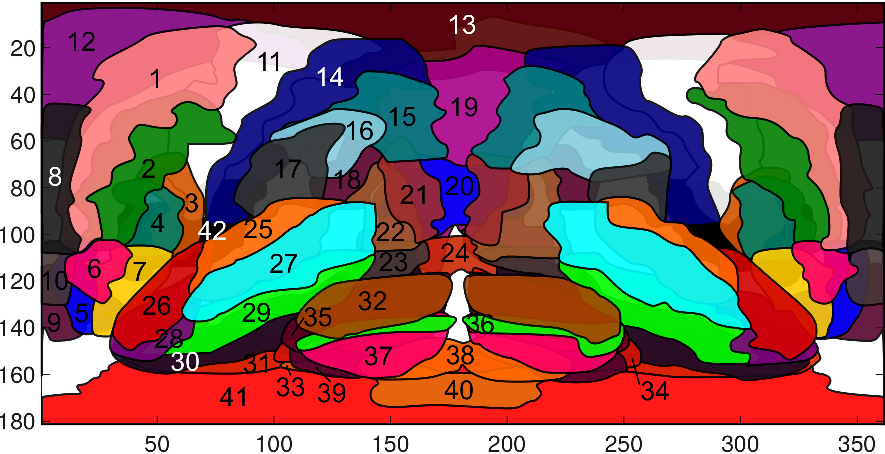
\includegraphics[width=0.7\textwidth]{Graphics/ch6/05-regions_cortical}
	
	\caption{Projection of different cortical regions. In the Frontal region, we can find: 1) Frontal Sup., 2) Frontal Mid., 3) Frontal Inf. Oper., 4) Frontal Inf. Tri., 5) Frontal Sup. Orb, 6) Frontal Mid. Orb, 7) Frontal Inf. Orb, 8) Frontal Sup. Medial, 9) Rectus, 10) Frontal Med. Orb., 11) Precentral, 12) Supp. Motor Area. In the Parietal region: 13) Paracentral Lobe, 14) Postcentral, 15) Parietal Sup., 16) Parietal Inf., 17) Supramarginal, 18) Angular. In the Occipital region: 19) Precuneus, 20) Cuneus, 21) Occipital Sup., 22) Occipital Mid., 23) Occipital Inf., 24) Lingual. In the Temporal region: 25) Temporal Sup., 26) Temporal Pole Sup., 27) Temporal Mid., 28) Temporal Pole Mid., 29) Temporal Inf, 30) Fusiform, 31) Parahippocampal. The Cerebellum, divided in: 32) Cerebelum Crus 1, 33) Cerebelum 3, 34) Cerebelum 4-5, 35) Cerebelum 6, 36) Cerebelum 7b, 37) Cerebelum 8, 38) Cerebelum 9, 39) Cerebelum 10. And additionally, the 40) Medulla, 41) Brain Stem and 42) Insula.}
	\label{fig:regionsCort}
\end{figure*}

\begin{figure*}[htp]
	\centering
	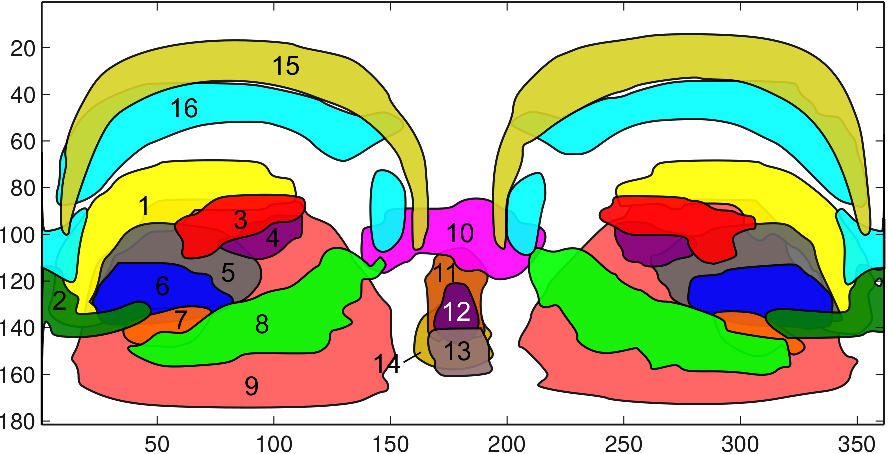
\includegraphics[width=0.7\textwidth]{Graphics/ch6/06-regions_subcortical}
	
	\caption{Projection of some important subcortical regions and organs. We observe the following subcortical structures: 1) Caudate Nucleus, 2) Olfactory Bulb, 3) Rolandic Operculum, 4) Heschl's gyri, 5) Putamen, 6) Globus Pallidus, 7) Amygdala, 8) Hippocampus, 9) Thalamus, 10) Lingual, 11) Vermis 4-5, 12) Vermis 7, 13) Vermis 9, 14) Vermis 1-2, 15) Cingulate Gyrus, 16) Corpus Callosum}
	\label{fig:regionsSub}
\end{figure*}

\subsubsection{Spherical Brain Mapping}\label{sec:sbmttest}
In this section, the six measures proposed in Section~\ref{sec:mapping} will be analysed using a $t$-test. To proceed, a $t$-value will be computed for each pixel in the maps, yielding a significance map. These significance maps, or $t$-maps, are presented in Figure~\ref{fig:tmaps}. 

\begin{figure*}[htp]
	\centering
	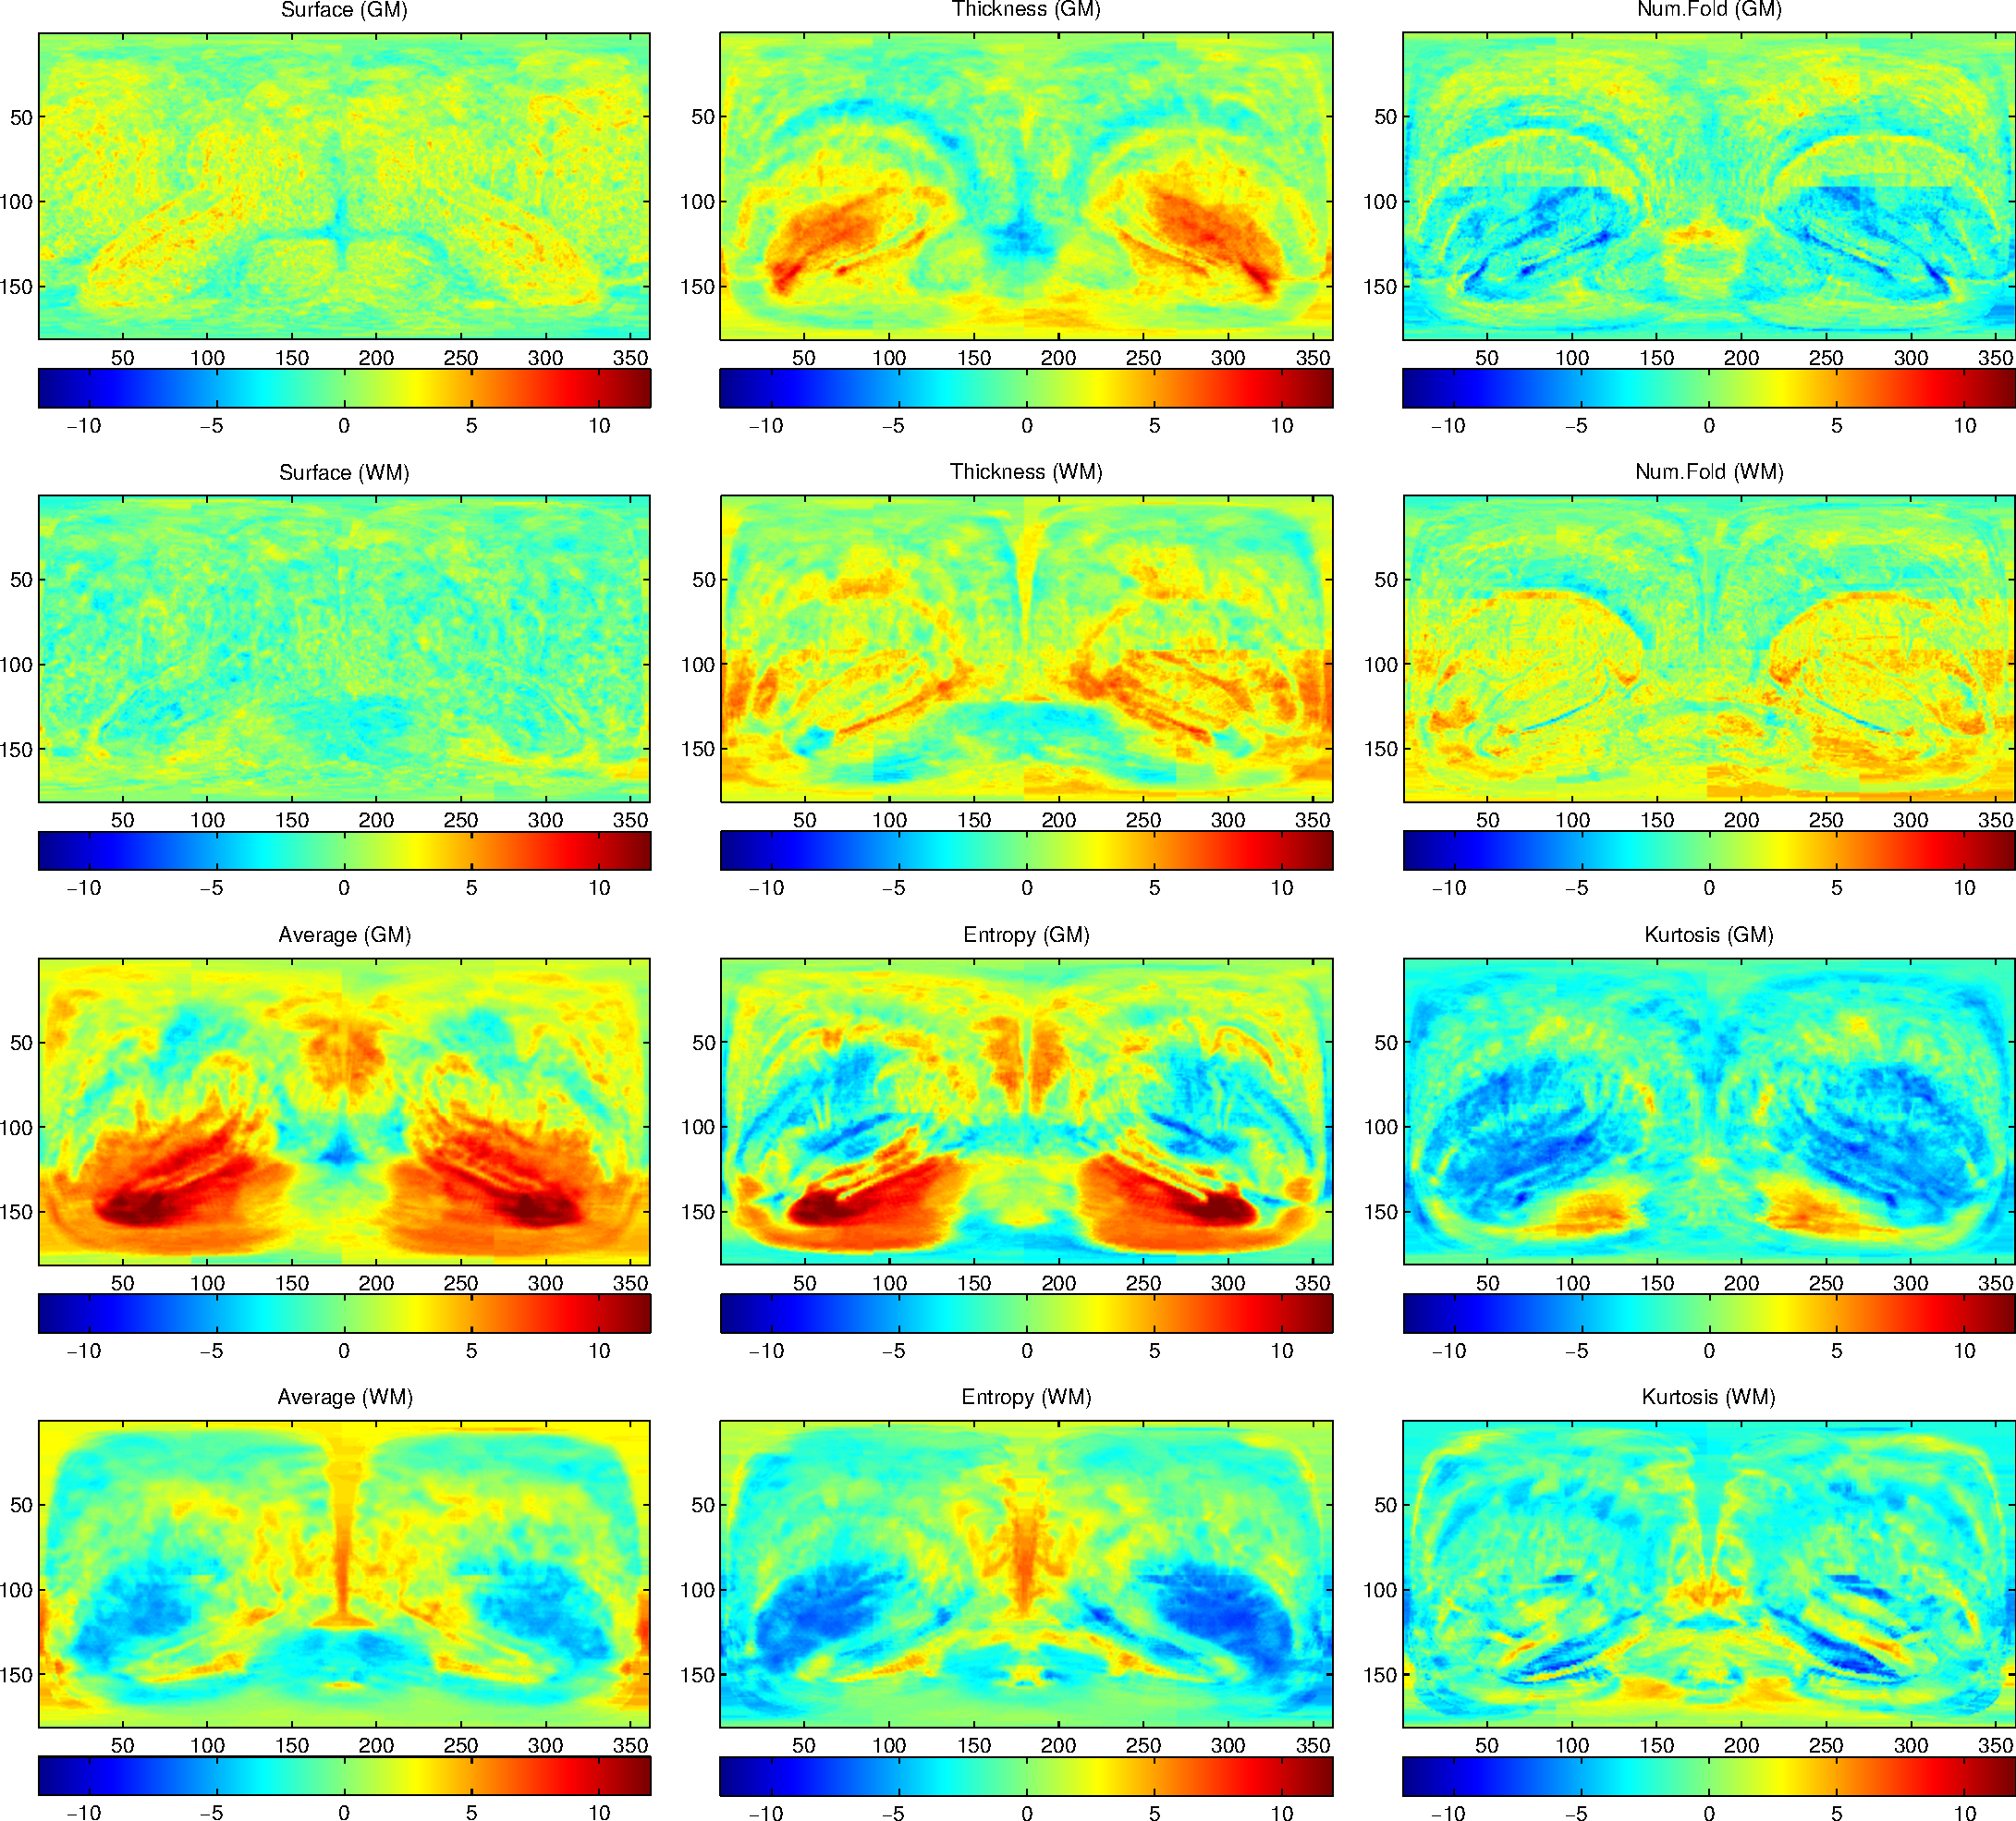
\includegraphics[width=0.9\textwidth]{Graphics/ch6/07-tmaps}
	\caption{$t$-maps that present the level of statistical relevance in the AD vs. NC paradigm, for each type of mapping and \ac{GM} and \ac{WM}. }
	\label{fig:tmaps}
\end{figure*}

Absolute $t$-values higher than $1.96$ can be considered to be significant, with a $p<0.05$. In this case the areas of greater significance are in dark red and dark blue, where red is a positive $t$-value, meaning a higher value in controls than in AD subjects, and blue is a negative $t$-value, and conversely, blue means negative values, which are related to a higher value in AD than in controls. 

The first thing to note is that the distribution of the $t$ values in the Surface mapping, in both \ac{GM} and \ac{WM}, is not relevant at all, with very few significant pixels distributed along the whole image. 

In the remaining \ac{GM} mappings, greater $t$-values are located in the frontal, occipital and parietal lobes, but the most significant areas can be found in the temporal lobe. This is most obvious in the Average and Entropy mappings, but can also be found in Thickness. Number of Folds and Kurtosis present high, but however negative, $t$-values in these areas as well. This suggests that for \ac{GM}, most of the neurodegeneration is located in the temporal lobe and all the underlying structures that are projected in this area, including the Hippocampus and Parahippocampal gyrus, which are considered a fundamental disease indicator in the NINCDS-ADRDA criteria \cite{Dubois2007}. Additionally, some structures that are located in the same area have been recently related to the progression of the disease, such as the Caudate Nucleus and Putamen \cite{Pievani2013}. These changes are more precisely located when using one of our spherical maps such as the Average or Entropy.

Conversely, in the \ac{WM} mappings the selected regions are different. When using Number of Folds and Thickness, the selected areas are located in the vicinity of those obtained in \ac{GM}. However, our spherical maps, especially Average and Entropy, behave differently. There is still high $t$-values that correspond to the White Matter of the Parahippocampal gyrus, but large areas of negative $t$-values that are located in areas corresponding to the Caudate Nucleus, Globus Pallidus and Putamen. The areas corresponding to the Posterior Cingulate gyrus and adjacent Precuneus present also values related to cell loss, as suggested in \cite{Baron2001}.

\subsubsection{Layered Extension}\label{sec:layeredttest}
The significance levels of the layered mappings has been assessed as well. However, due to space restrictions, we will only analyse the anatomical features of one of the mappings: a four-layered average mapping of the \ac{GM}, that can be checked in Figure~\ref{fig:tmaplayered}.

\begin{figure*}[htp]
	\centering
	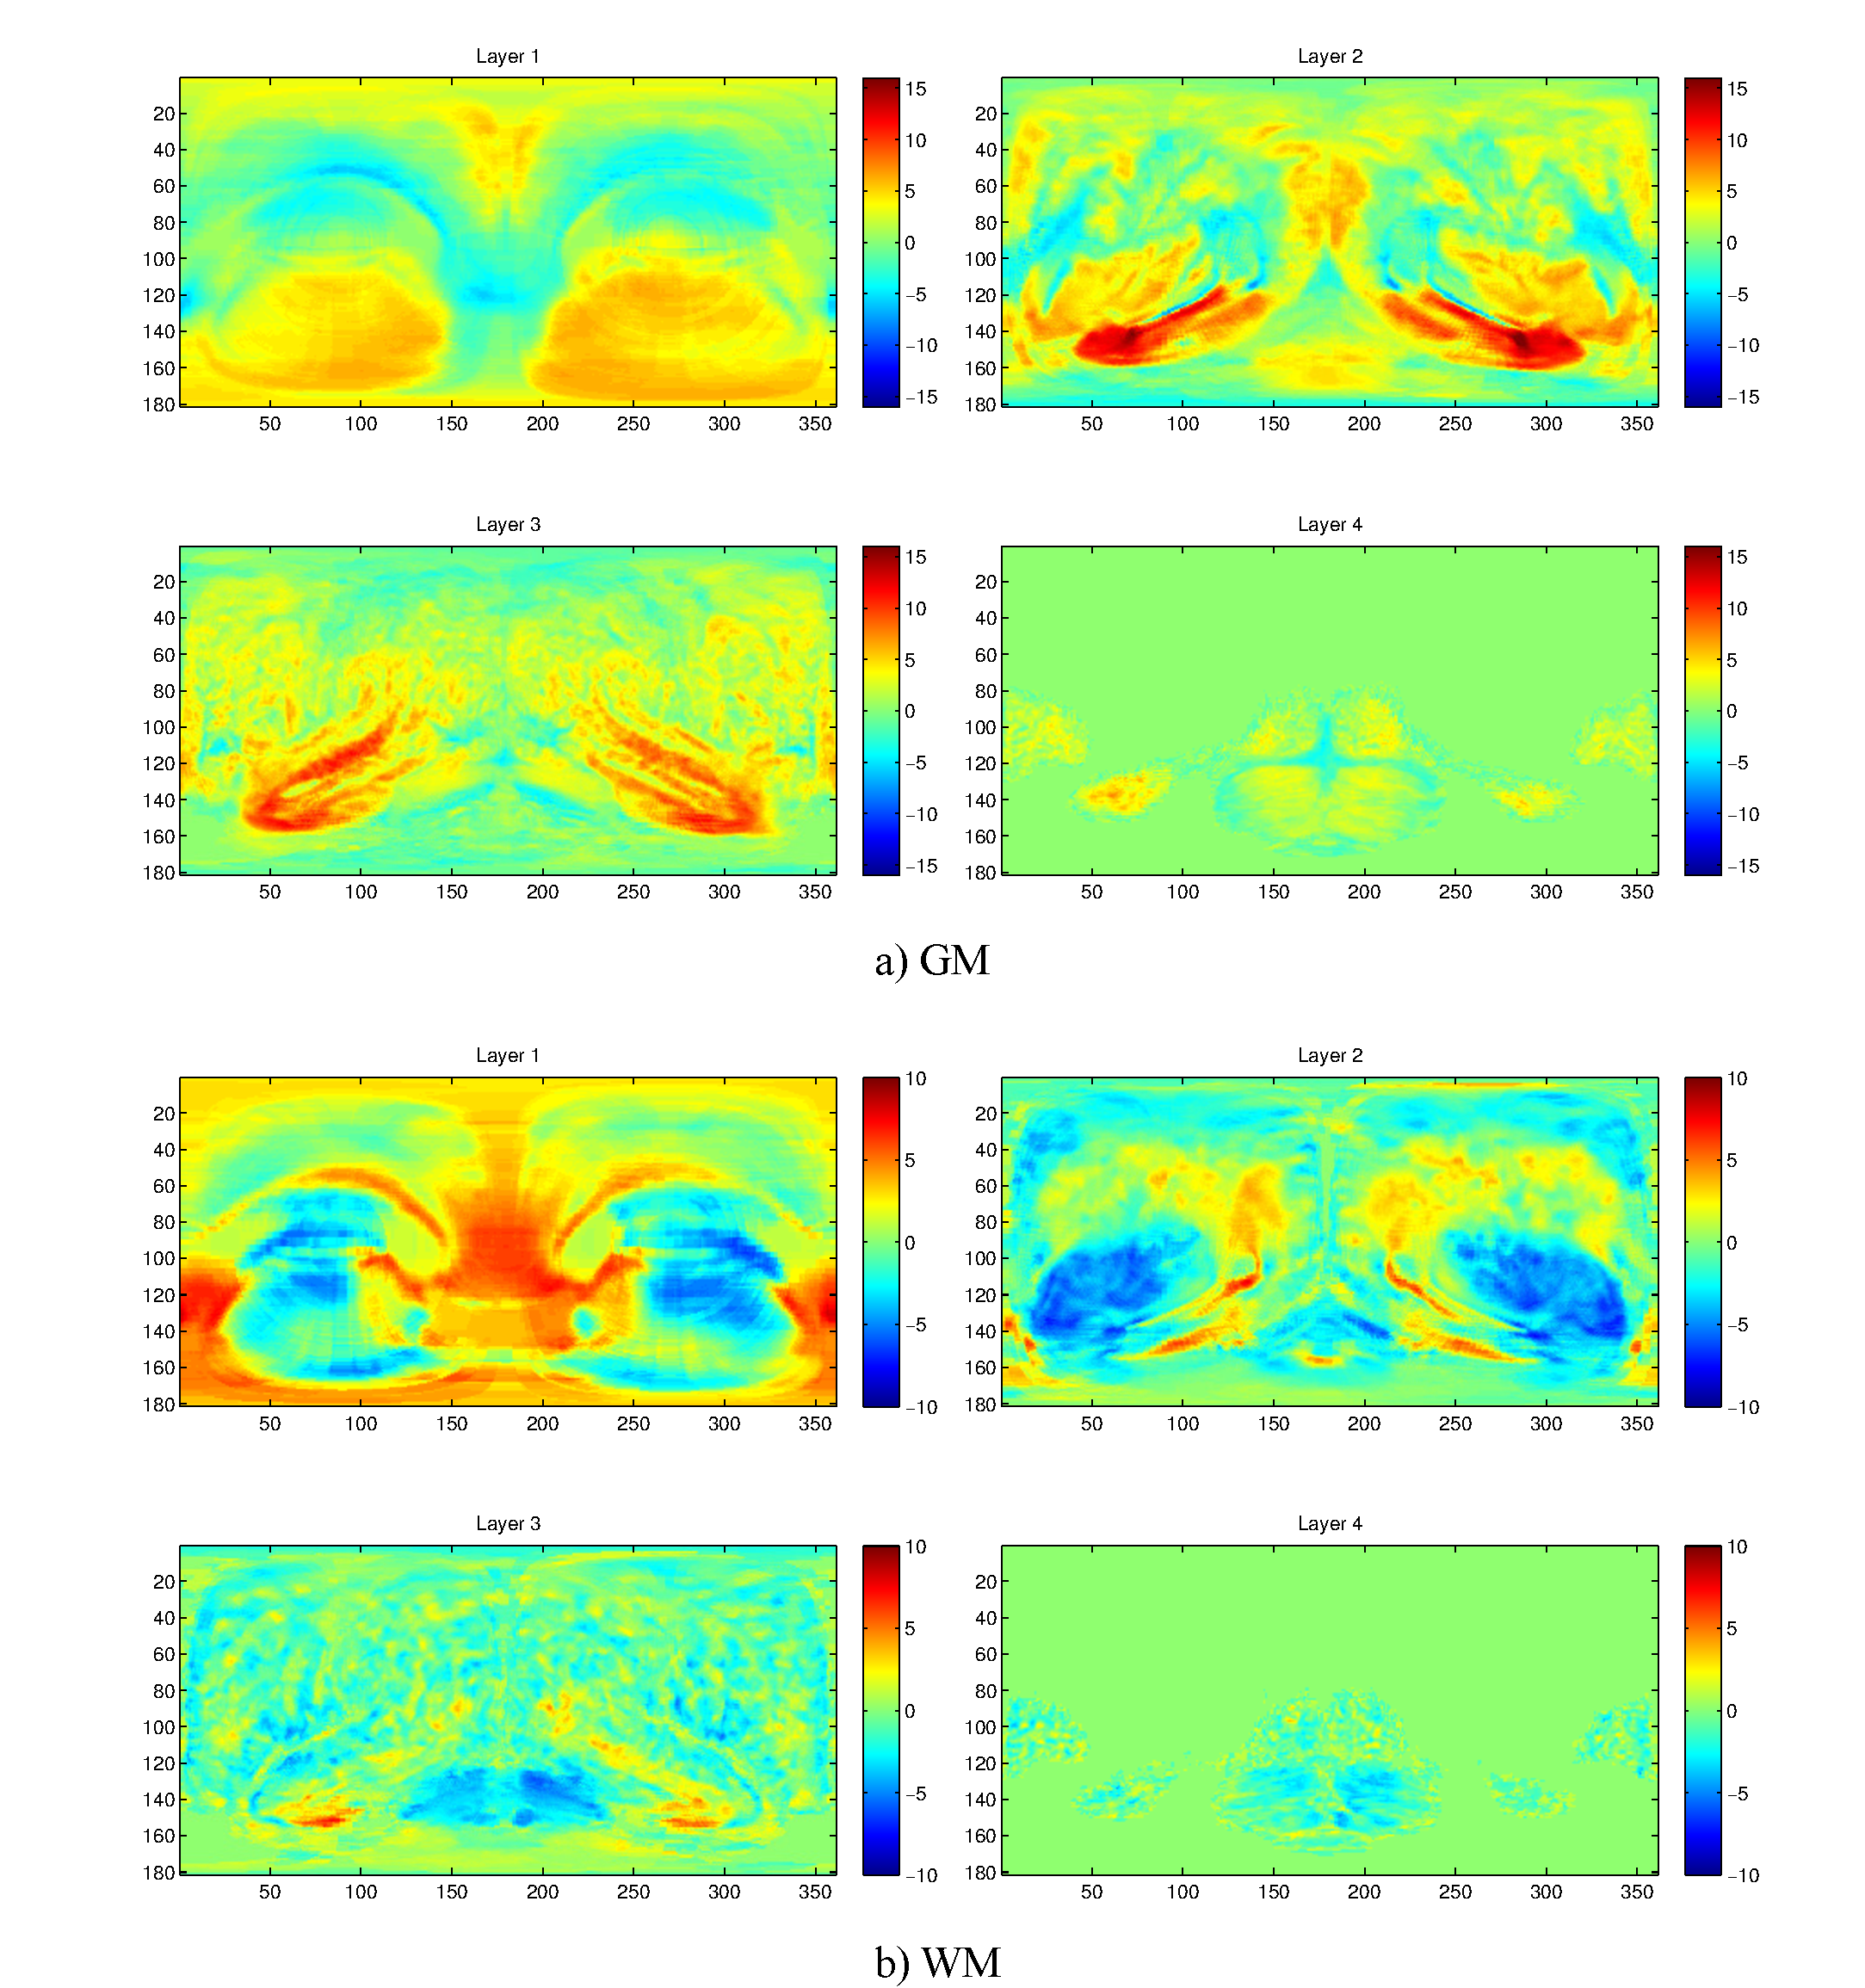
\includegraphics[width=\textwidth]{Graphics/ch6/08-Tmap4LayAverage}
	\caption{$t$-maps that present the level of statistical relevance in the AD vs. NC paradigm, for a four-layered average mapping over a) \ac{GM} and b) \ac{WM}. }
	\label{fig:tmaplayered}
\end{figure*} 

It is plain to see that most of the neurological changes in \ac{GM} appear in layers 2 and 3, specifically in the Hippocampus, Parahippocampal lobe and Amygdala (layer 2) and the temporal lobe (layer 3), where the values of the average mapping (equivalent to the density of the tissue) are higher in normal control subjects than in AD affected patients. This reveals atrophy in these organs, as it has been previously reported in the bibliography \cite{Dubois2007,Pievani2013}. In the case of \ac{WM}, however, the changes are negative in the areas where the Rolandic Operculum, Heschl's gyri, Putamen and Globus Pallidus are found, and positive in some sections of the Hippocampus and the White Matter contained in the Parahippocampal lobe and the remaining parts of temporal lobe (layer 2 and 3). Nevertheless, the most significant differences are located in layer 1, in the borders between ventricles and Thalamus, and specially in the Cuneus, Precuneus and Posterior Cingulate gyrus, which were reported in \cite{Baron2001}. 

\subsubsection{VRLBP}\label{sec:vrlbpttest}
Finally, to end this statistical significance analysis, the $t$-maps of the more complex VRLBP mapping are presented in Figure~\ref{fig:tmapvrlbp}.

\begin{figure*}[htp]
	\centering
	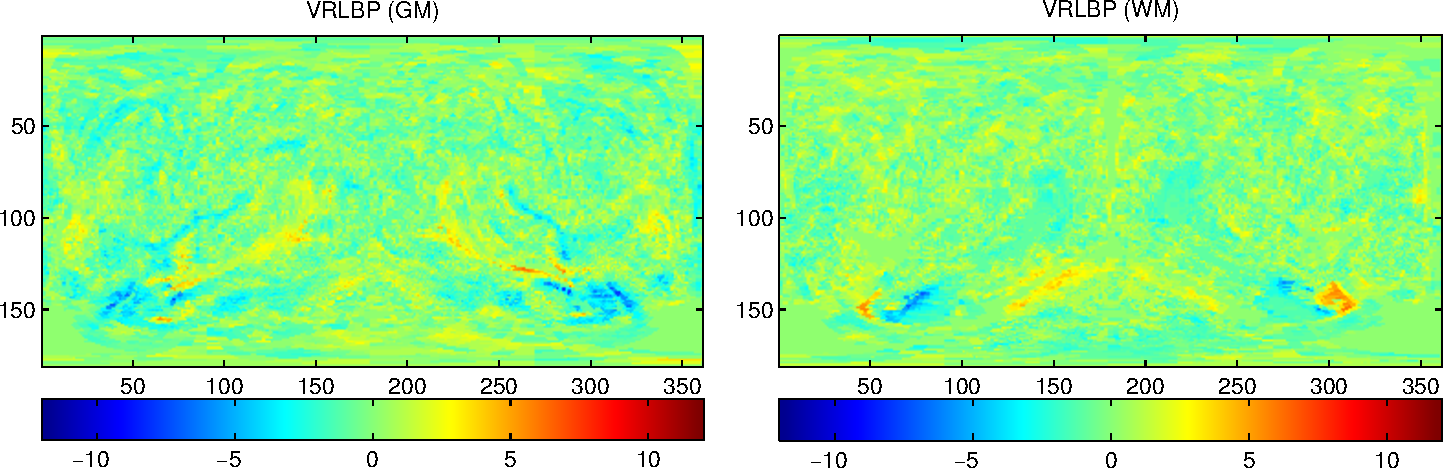
\includegraphics[width=\textwidth]{Graphics/ch6/09-tmaps_vrlbp}
	\caption{$t$-maps that present the level of statistical relevance in the AD vs. NC paradigm, for the VRLBP projections mapping over a) \ac{GM} and b) \ac{WM}. }
	\label{fig:tmapvrlbp}
\end{figure*}

These maps present low absolute $t$ levels in most of the projection, however some small regions present high significance. These regions correspond to small areas in temporal lobe, Amygdala and Hippocampus in the \ac{GM}, and even smaller regions in the \ac{WM} corresponding to the limits between Hippocampus and Amygdala. 

\subsection{Classification Analysis}\label{sec:classification}
To obtain comparable performance metrics suitable to analyse the generalization capabilities of \ac{SBM}, in this section a number of classification results are presented. A baseline is established in Section~\ref{sec:baseline} and then the performance of our maps, included the layered extension and VRLBP, is presented in Section~\ref{sec:sbmclass}.

\subsubsection{Baseline - VAF}\label{sec:baseline}
In order to establish a baseline to assess the predictive ability of our maps, we will use the \acf{VAF} paradigm, described in \cite{Stoeckel04}. This approach uses the whole 3D \ac{GM} or \ac{WM} segmented MR images and then uses all voxels of the 3D images as features in the SVM classification, yielding the performance values shown in Table~\ref{tab:perfVAF}. The performance of the \ac{SBM} maps will be compared to these. 

\begin{table*}[htp]
	\myfloatalign
	\begin{tabularx}{\textwidth}{Xccc}
		\tableheadline{Approach}  & \tableheadline{Accuracy} & \tableheadline{Sensitivity} & \tableheadline{Specificity}\\
		\midrule
		\ac{VAF} (\ac{GM})  & $0.768 \pm 0.011$ & $0.752 \pm 0.016$ & $0.785 \pm 0.016$ \\
		\ac{VAF} (\ac{WM})  & $0.642 \pm 0.009$ & $0.668 \pm 0.012$ & $0.617 \pm 0.013$ \\
		\bottomrule
	\end{tabularx}
	\caption{Performance values (Average $\pm$ Standard Deviation) for the  Voxels as Features approach in both \ac{GM} and \ac{WM} tissues.\label{tab:perfVAF}}
\end{table*}

\subsubsection{Spherical Brain Mapping}\label{sec:sbmclass}
In this analysis, we have proceed as commented before, by computing the significance of each pixel using a $t$-test and then selecting a proportion of the most relevant, once they have been ranked according to their $t$-value. Later, these features are used to train and test a linear SVM classifier.

\begin{table*}[htp]
	\myfloatalign
	\begin{tabularx}{\textwidth}{Xcccc}
		\tableheadline{Approach} & \tableheadline{Perc.} & \tableheadline{Accuracy} & \tableheadline{Sensitivity} & \tableheadline{Specificity}\\
		\midrule
		Surface (\ac{GM}) & $0.100$ & $0.638 \pm 0.006$ & $0.660 \pm 0.030$ & $0.616 \pm 0.024$ \\
		Surface (\ac{WM}) & $0.100$ & $0.672 \pm 0.007$ & $0.692 \pm 0.018$ & $0.652 \pm 0.018$ \\
		\midrule
		Thickness (\ac{GM})  & $0.725$ & $0.781 \pm 0.007$ & $0.811 \pm 0.011$ & $0.751 \pm 0.017$ \\
		Thickness (\ac{WM}) & $0.925$ & $0.758 \pm 0.009$ & $0.773 \pm 0.017$ & $0.744 \pm 0.011$ \\
		\midrule
		Num.Fold (\ac{GM}) & $0.600$ & $0.749 \pm 0.013$ & $0.782 \pm 0.019$ & $0.716 \pm 0.013$ \\
		Num.Fold (\ac{WM}) & $0.500$ & $0.757 \pm 0.005$ & $0.745 \pm 0.006$ & $0.768 \pm 0.009$ \\
		\midrule
		Average (\ac{GM}) & $0.575$ & $0.879 \pm 0.005$ & $0.897 \pm 0.006$ & $0.861 \pm 0.006$ \\
		Average (\ac{WM}) & $0.150$ & $0.800 \pm 0.011$ & $0.802 \pm 0.013$ & $0.798 \pm 0.009$ \\
		\midrule
		Entropy (\ac{GM}) & $0.825$ & $0.846 \pm 0.008$ & $0.842 \pm 0.009$ & $0.849 \pm 0.011$ \\
		Entropy (\ac{WM}) & $0.525$ & $0.796 \pm 0.006$ & $0.811 \pm 0.009$ & $0.781 \pm 0.009$ \\
		\midrule
		Kurtosis (\ac{GM}) & $1.000$ & $0.753 \pm 0.007$ & $0.801 \pm 0.011$ & $0.704 \pm 0.015$ \\
		Kurtosis (\ac{WM}) & $0.175$ & $0.697 \pm 0.008$ & $0.702 \pm 0.018$ & $0.693 \pm 0.009$ \\
		\midrule
		VRLBP (\ac{GM}) & $0.200$ & $0.903 \pm 0.010$ & $0.890 \pm 0.012$ & $0.916 \pm 0.018$ \\
		VRLBP (\ac{WM}) & $0.150$ & $0.909 \pm 0.014$ & $0.899 \pm 0.028$ & $0.919 \pm 0.018$ \\
		\bottomrule
	\end{tabularx}
	\caption{Performance values (Average $\pm$ Standard Deviation) for the different \ac{SBM} approaches.}
	\label{tab:perfProj}
\end{table*}

The results for each type of map are presented in Table~\ref{tab:perfProj}, including the percentage of selected voxels (perc.) at which each value is obtained. Regarding the Grey Matter, we can observe that the best type of mappings in the diagnosis task, in terms of average accuracy, are the Average ($0.879 \pm 0.005$) and Entropy ($0.846 \pm 0.008$). There results are followed by the measures of Thickness ($0.781 \pm 0.007$), Kurtosis ($0.753 \pm 0.019$) and the worse accuracy estimates are for Number of Folds ($0.749 \pm 0.013$) and Surface ($0.638 \pm 0.006$). 

In the case of White Matter, and according to Table~\ref{tab:perfProj}, the performance is again higher in Average ($0.800 \pm 0.011$) and Entropy ($0.796 \pm 0.006$). Thickness and Number of Folds present similar, but lower, perfomance values, respectively $0.758 \pm 0.009$ and$0.757 \pm 0.005$, and being the Kurtosis ($0.697 \pm 0.008$) and Surface ($0.672 \pm 0.007$) maps the less powerful. 

However, VRLBP outperform all these approaches by obtaining an accuracy of $0.903 \pm 0.010$ for \ac{GM} and $0.909 \pm 0.014$ for \ac{WM}, revealing itself as the best technique. 

The evolution of the performance of the maps as the number of selected pixels varies is shown in Figure~\ref{fig:figureGM}. In general, it is possible to see very small differences in the accuracy of the system, which makes its performance almost independent from the number of selected pixels. However, this is not the case of the Surface, and, more remarkable, the VRLBP. In the latter, the performance is the best for both tissues when the proportion of selected pixels is small, but degrades significantly as its number increases. 

\begin{figure*}[htp]
	\centering
	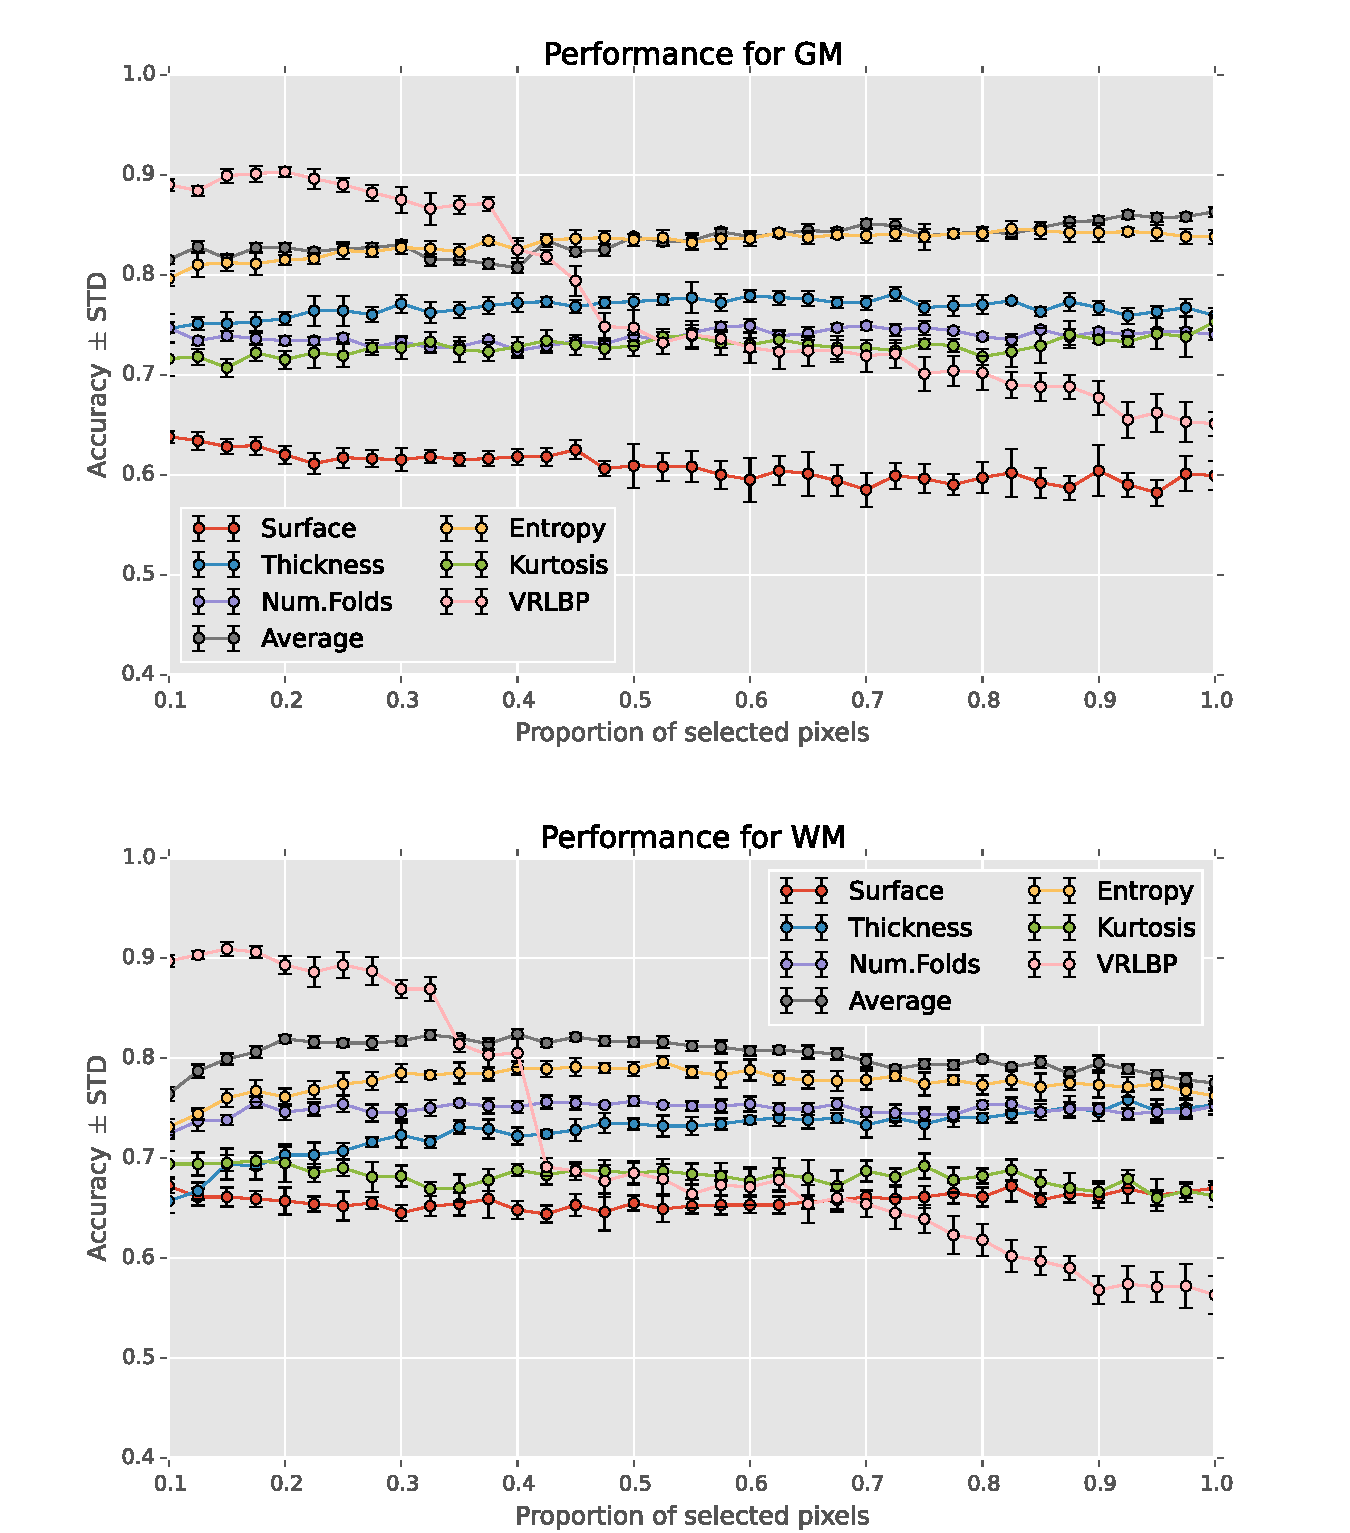
\includegraphics[width=0.9\textwidth]{Graphics/ch6/10-comparisonPerformance}
	\caption{Performance for the different \ac{SBM} approaches over the: a) Grey Matter and b) White Matter.}
	\label{fig:figureGM}
\end{figure*}

Regarding the four-layer extension to \ac{SBM}, the performance values obtained by different mappings at different layers and thresholds ($t$-values of 2, 4, 8 and 10) is presented in Figure~\ref{fig:layeredPerf}. 

\begin{figure*}[htp]
	\centering
	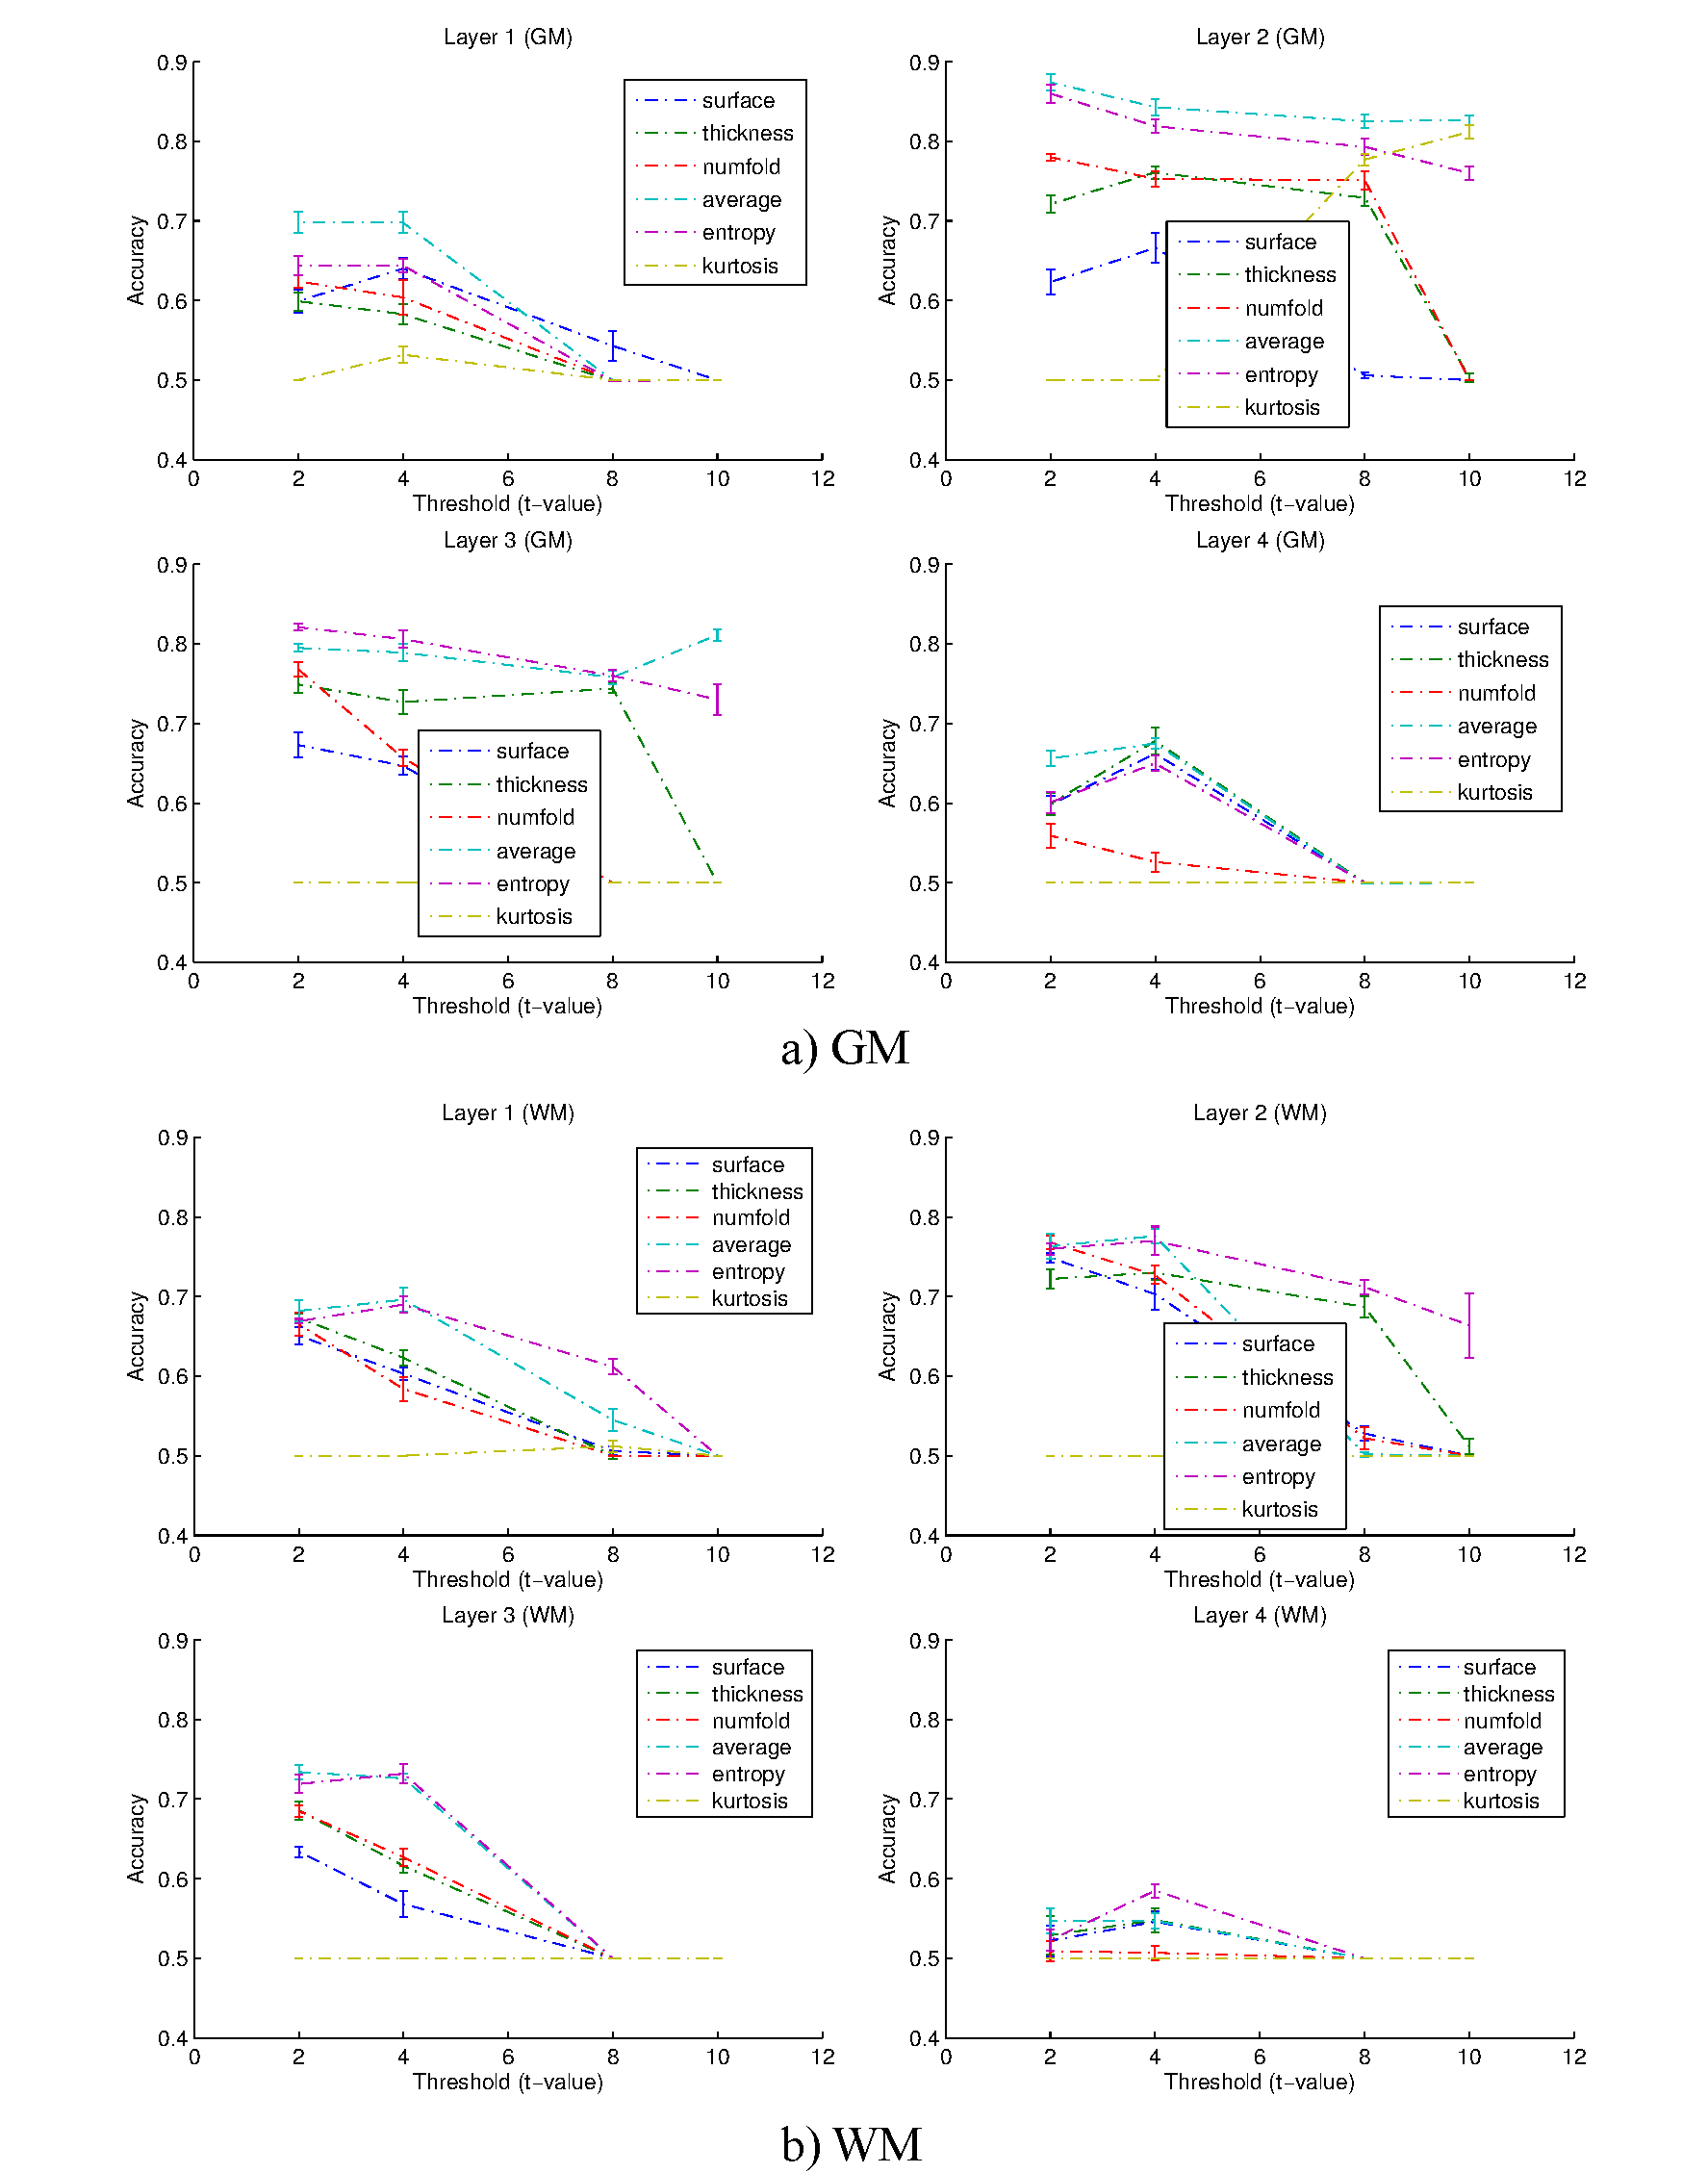
\includegraphics[width=0.9\textwidth]{Graphics/ch6/11-layerPerf}
	\caption{Performance for the different four-layered mappings over the: a) Grey Matter and b) White Matter at different levels of statistical significance.}
	\label{fig:layeredPerf}
\end{figure*}

The first thing that we can observe is that for both \ac{GM} and \ac{WM} tissues, the better performance is achieved with the second layer. This is specially surprising in the \ac{WM} case, as the highest $t$-values were located in layer 1. 

\subsection{Experimental Setup}
In order to test our \ac{HMM}-based path tracing algorithm, we propose the following experiments: 
\begin{itemize}
	\item Firstly, in Sec.~\ref{sec:demo} an evaluation of the algorithm over two synthetic 2D and 3D images. 
	\item Secondly, in Sec.~\ref{sec:intensity}, the \ac{HMM} paths created using the DARTEL template will be evaluated in the differential diagnosis (NC versus AD). 
	\item Finally, in Sec.~\ref{sec:texture}, the proposed texture feature maps computed along the DARTEL \ac{HMM} paths will be evaluated in a differential diagnosis as well. 
\end{itemize}

For sections \ref{sec:intensity} and \ref{sec:texture} a similar strategy is used to obtain performance results. Once a set of features has been extracted (intensity values in each path and statistical measures for Section~\ref{sec:intensity} and texture features for Section~\ref{sec:texture}), they are used to train and classify a Support Vector Machine (SVM) classifier with linear kernel, as implemented in \texttt{LIBSVM}\cite{Chang2001}, to classify the component scores. The classification was validated using stratified 10-fold cross-validation, as recommended in \cite{Kohavi1995a}.

\subsection{2D and 3D demonstrations}\label{sec:demo}
A demonstration of the ability of our \ac{HMM} path tracing algorithm can be found in Figures~\ref{fig:gaussian} and \ref{fig:spire}. In Fig.~\ref{fig:gaussian}, the path tracing algorithm has been tested over a synthesized gaussian mixture probability density function using four isotropic gaussian kernels. The initial point was located at $\mathbf{x}_0 = (120,20)$ and the attractor at $\mathbf{x}_N = (20, 60)$. The resulting path maximizes both the orientation of the path (towards $\mathbf{x}_N$) and the minimum change in the intensity values, which is specially visible in the last nodes of the path, where it approaches $\mathbf{x}_N$ surrounding the nearby kernel. In this case, the chosen L2-norm of the support ball has been $r=3$. 
\begin{figure}
	\begin{center}
		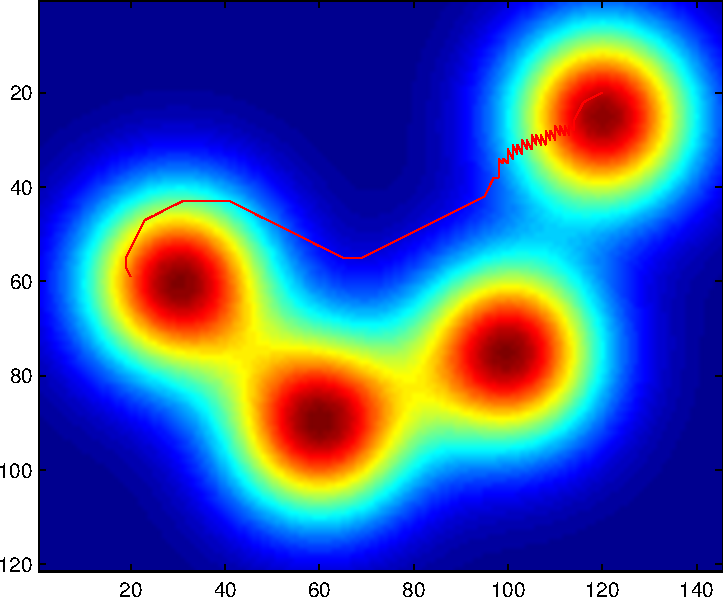
\includegraphics[width=1.5in]{Graphics/ch6/gaussian}
		\caption{Path traced over a gaussian mixture distribution of 4 isotropic gaussian kernels.}
		\label{fig:gaussian}
	\end{center}
\end{figure}

The algorithm has been tested on a three-dimensional, helix-shaped point distribution as well (Fig.~\ref{fig:spire}). The tracing algorithm needs per-voxel intensity (or probability) values, therefore we have estimated the probability distribution of the points as the number of points within each voxel over the total number of points. Using $\mathbf{x}_0$ as the point with minimum $z$ coordinate in the data distribution and $\mathbf{x}_N$ the one with maximum $z$, the resulting path follows the data distribution consistently until it reaches the attractor. 
\begin{figure}
	\begin{center}
		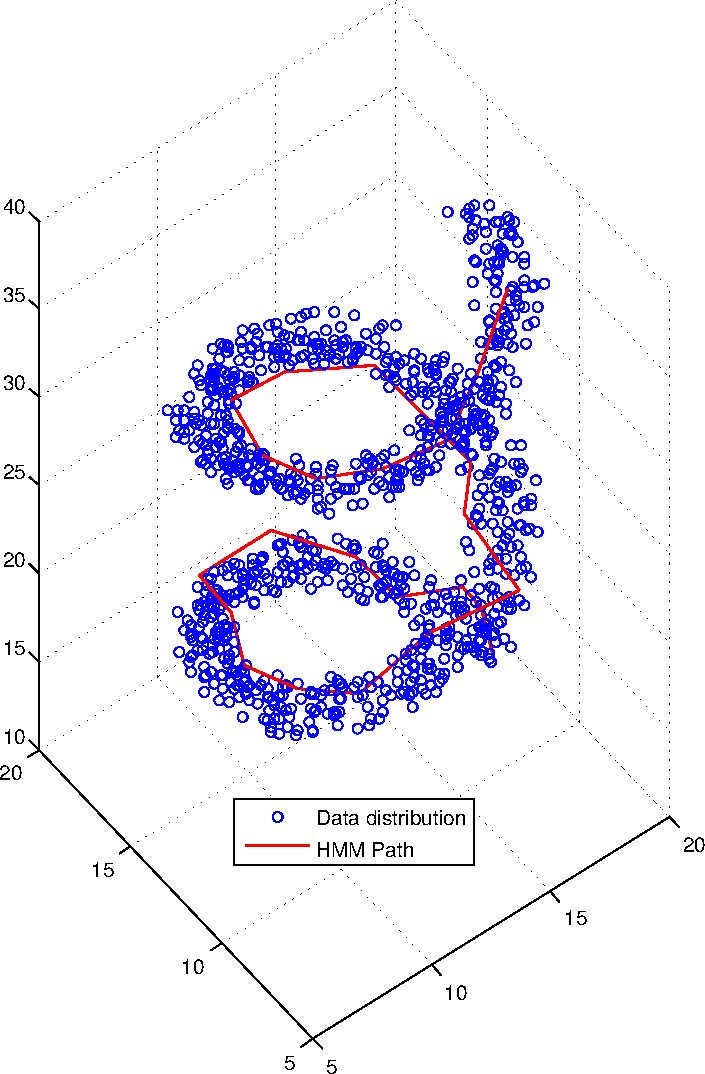
\includegraphics[width=1.5in]{Graphics/ch6/spire}
		\caption{\ac{HMM} path computed inside a density distribution defined by an helix.}
		\label{fig:spire}
	\end{center}
\end{figure}

Finally, we have tested the algorithm on a real world example, using a digital elevation model (DEM) of the Iberian Peninsula, generated by the LANDSAT SRTM30+ mission (see Fig.~\ref{fig:spainmap}). We have tested a multiple path tracing by establishing sequentially $\mathbf{x}_0$ and $\mathbf{x}_N$ in ten cities. The resulting paths optimize both the distance and height variation, as well as resembling -in most cases- the roads that connect these cities in the real world. Given the dimensions of the image, in this case, the L2-norm of the support ball has been set to $r=30$. 

\begin{figure}[htp]
	\centering
	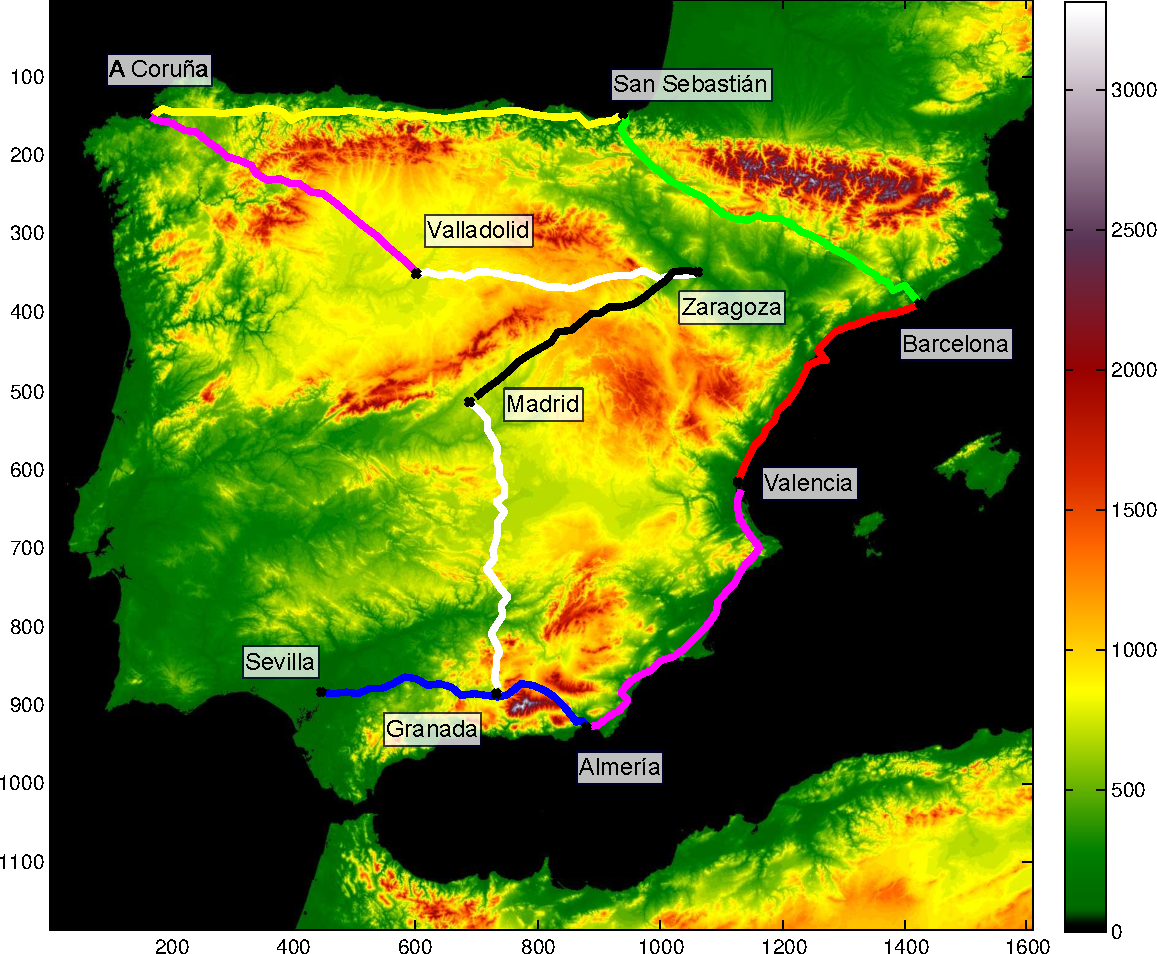
\includegraphics[width=0.7\textwidth]{Graphics/ch6/spain.pdf}
	\caption{Simulation of the \ac{HMM}-based path tracing over an Iberian Peninsula height map, interconecting different cities.}
	\label{fig:spainmap}
\end{figure}



\subsection{Intensity paths}\label{sec:intensity}
In this section, we present the results of the first experiment involving paths in MRI. To do so, we define a set of canonical paths that are computed on the DARTEL template. These DARTEL paths model the anatomy of a normal subject to whom all other images have been registered. This means that we have fixed the location of the nodes to the structural information of the template, and by extension, to the general anatomy of all images in the database. Therefore, we can characterize the structural differences by the intensity distribution --in other words, the tissue density--  of the voxels at the path nodes. Comparing the intensity distribution found in controls to the one found in AD affected subjects is thus the first logical step to measure how these paths can distinguish the different classes.

To test the algorithm we use the $180\times360=64800$ DARTEL paths computed in each spatial direction $(\varphi,\theta)$, with $\varphi\in[0,360]$ and $\theta\in[-90,90]$, to select the intensities in the voxels that are placed at the nodes. The amount of voxels selected ranges from 2 to several dozens. The set of selected intensities are used as features to train and test a SVM classifier. The accuracy reached by each path (using the aforementioned cross-validation strategy) is presented as colour information in Figure~\ref{fig:accuracyMap}. The higher accuracy obtained using only one path is $0.8028\pm0.0873$, and corresponds to the light green paths that cross the temporal lobe. 

\begin{figure}
	\begin{center}
		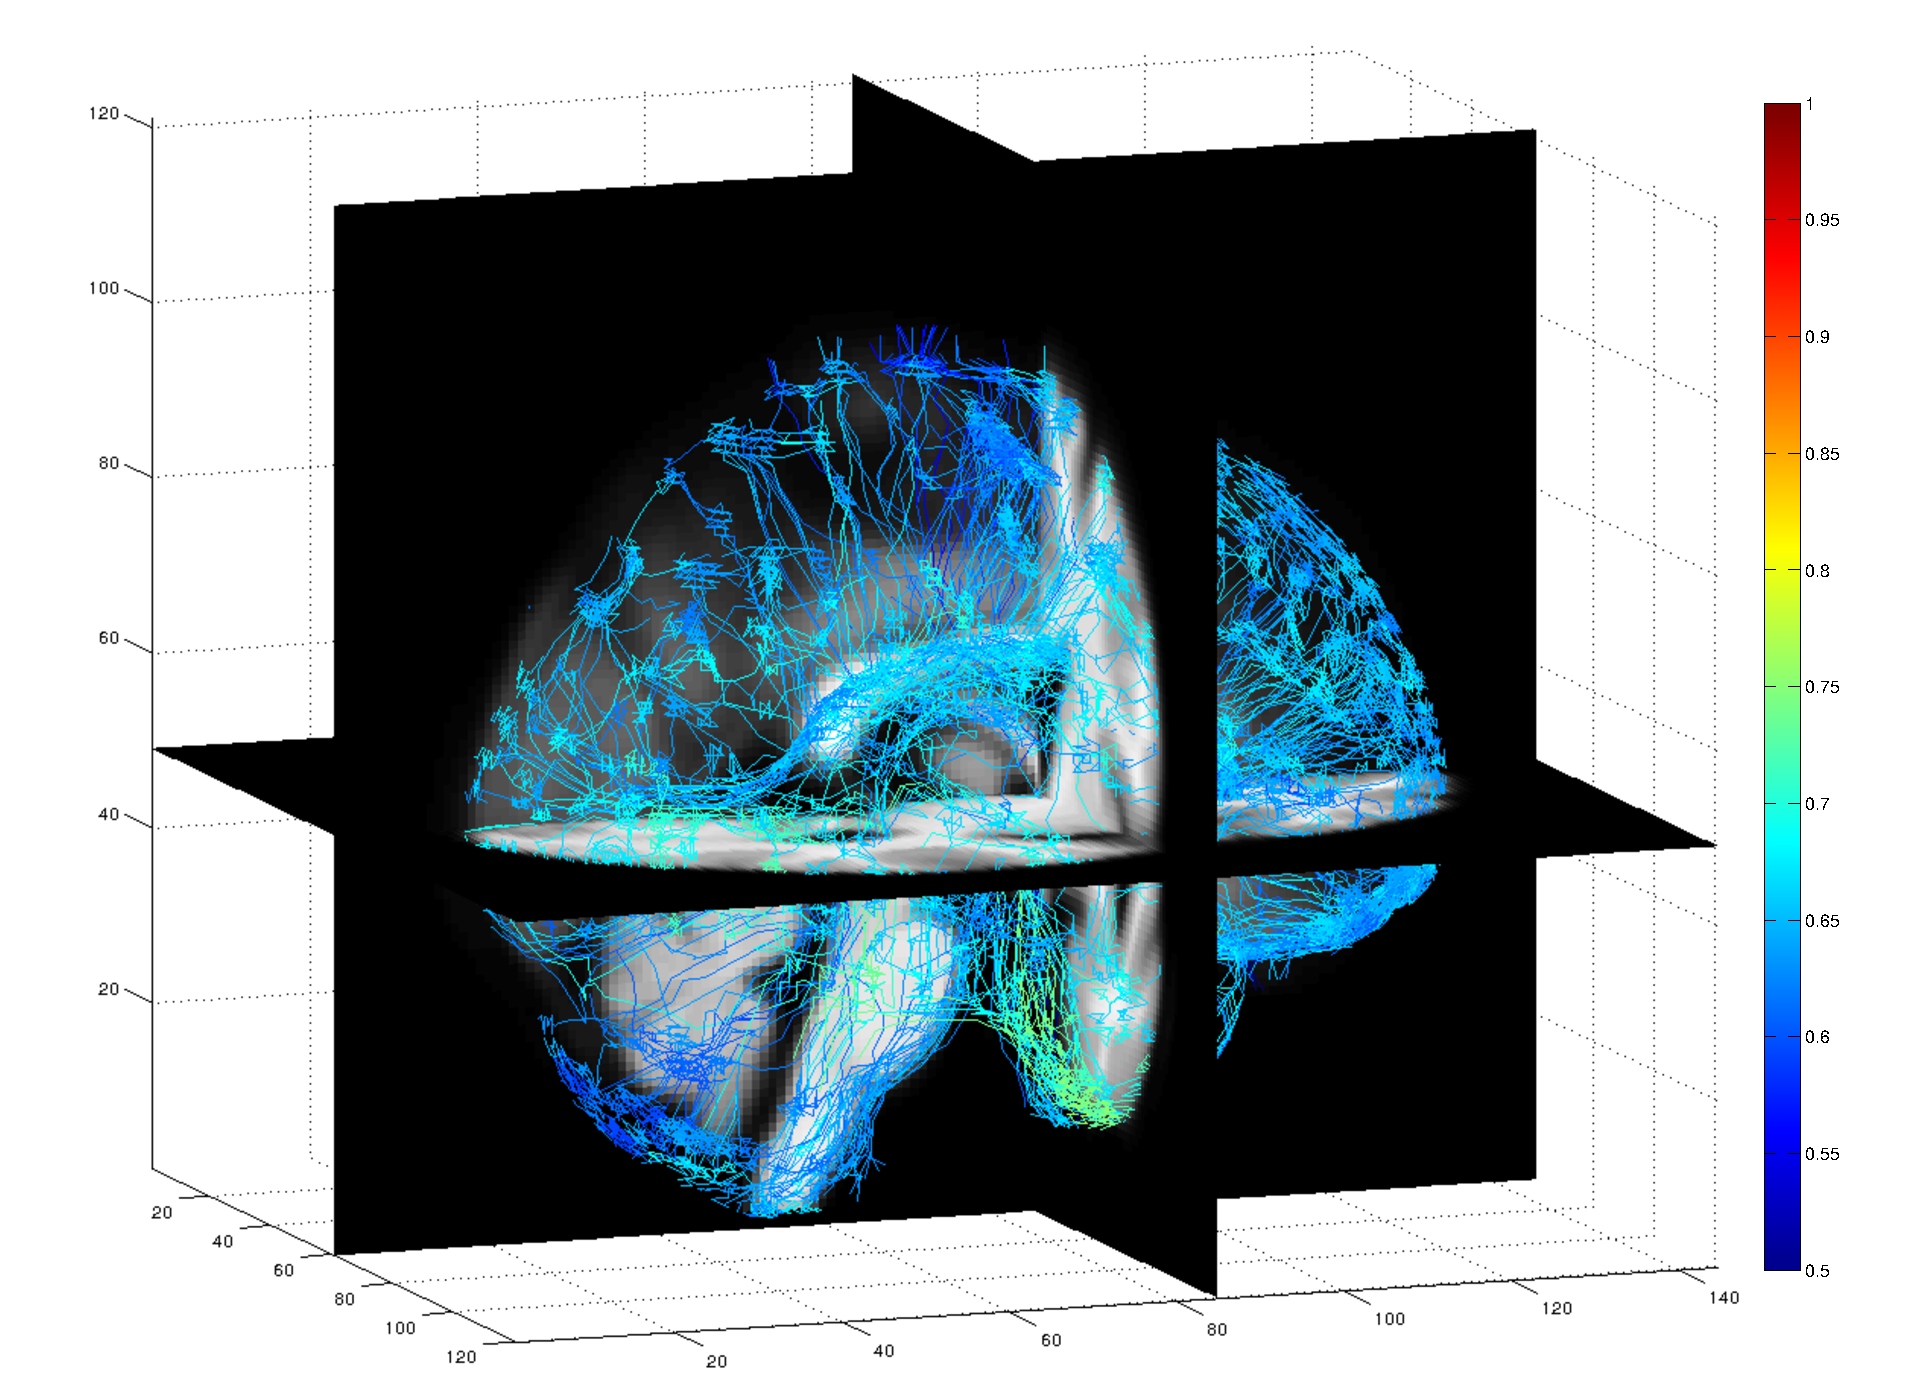
\includegraphics[width=\columnwidth]{Graphics/ch6/accuracyPaths2}
		\caption{DARTEL paths computed in each direction ($\varphi,\theta$). Each path's colour represent the accuracy in a differential diagnosis. Only one in every five paths are shown for clarity purposes.}
		\label{fig:accuracyMap}
	\end{center}
\end{figure}

It is interesting to question if the performance of this differential diagnosis could be improved using the information contained in more than one path at a time. To this end, we first take the higher accuracy ($\text{accuracy} \ge0.7$) paths according to the aforementioned performance and select all voxels located in the nodes of these paths. Additionally, we use a $t$-test over the set of voxels selected by these paths, to further reduce the set to those voxels that have significant ($p<0.05$) $t$-values ($|t|>1.96$). The performance values for the experiment involving all voxels in the paths (first row) and the one that uses only those significant voxels (second row) are presented in Table~\ref{tab:acc}. 

\begin{table}
	\myfloatalign
	\begin{tabularx}{\textwidth}{Xccc}
		\tableheadline{Side} & \tableheadline{Accuracy} & \tableheadline{Sensitivity} & \tableheadline{Specificity} \\ \midrule
		Both & $0.806 \pm 0.069 $ & $0.733 \pm 0.073$ & $0.878 \pm 0.097$\\
		Left & $0.769 \pm 0.035 $ & $0.717 \pm 0.061$ & $0.822 \pm 0.057$\\
		Right & $0.792 \pm 0.080 $ & $0.706 \pm 0.120$ & $0.878 \pm 0.101$\\
		\midrule 
		Both & $0.828 \pm 0.054 $ & $0.794 \pm 0.095$ & $0.861 \pm 0.039$\\
		Left & $0.733 \pm 0.037 $ & $0.694 \pm 0.099$ & $0.772 \pm 0.124$\\
		Right & $0.781 \pm 0.085 $ & $0.711 \pm 0.122$ & $0.850 \pm 0.083$\\
		\bottomrule
	\end{tabularx}
	\caption{Performance values ($\pm$SD) for the selected paths as features, and using $t$-test to select the voxels.} 
	\label{tab:acc}
\end{table}

Finally, we mimic the procedure followed in the \ac{SBM} article\cite{Martinez-Murcia2015}. That is, we first compute the average, variance, entropy and kurtosis maps of each brain, but instead of using rectilinear paths, we use the DARTEL paths. Afterwards, all the features contained in these maps are used as an input to the SVM classifier. The performance results are shown in Table~\ref{tab:sbm_perf}. 

\begin{table}
	\myfloatalign
	\begin{tabularx}{\textwidth}{Xccc}
		\tableheadline{Feature} & \tableheadline{Accuracy} & \tableheadline{Sensitivity} & \tableheadline{Specificity} \\ \midrule
		Average & $0.594 \pm 0.062 $ & $0.661 \pm 0.121$ & $0.528 \pm 0.106$\\
		Variance & $0.750 \pm 0.064 $ & $0.633 \pm 0.131$ & $0.867 \pm 0.102$\\
		Entropy & $0.603 \pm 0.069 $ & $0.661 \pm 0.071$ & $0.544 \pm 0.125$\\
		Kurtosis & $0.756 \pm 0.105 $ & $0.733 \pm 0.165$ & $0.778 \pm 0.150$\\
		\bottomrule
	\end{tabularx}
	\caption{Performance values ($\pm$SD) for each of the measures used in the \ac{SBM} article.} 
	\label{tab:sbm_perf}
\end{table}

\subsection{Texture features}\label{sec:texture}
The second experiment is intended to extract texture features from the DARTEL paths. With this approach, we obtain one single value per texture feature and path in the subjects, values that intrinsically contain information from their location in the path, in contrast to standard \ac{SBM} measures. In the end, each subject will be characterized by a 2D, $361\times181$ array of scalars, one for each texture feature applied to the paths. Performance values for the nine texture features maps from Section~\ref{sec:rtextfeat} are presented in Table~\ref{tab:texture}.

\begin{table*}
	\myfloatalign
	\begin{tabularx}{\textwidth}{Xccc}
		\tableheadline{Feature} & \tableheadline{Accuracy} & \tableheadline{Sensitivity} & \tableheadline{Specificity} \\ \midrule
		Contrast & $0.733 \pm 0.060 $ & $0.689 \pm 0.126$ & $0.778 \pm 0.105$\\
		Correlation & $0.672 \pm 0.068 $ & $0.672 \pm 0.112$ & $0.672 \pm 0.100$\\
		Dissimilarity & $0.711 \pm 0.085 $ & $0.678 \pm 0.110$ & $0.744 \pm 0.102$\\
		Energy & $0.689 \pm 0.061 $ & $0.700 \pm 0.115$ & $0.678 \pm 0.073$\\
		Entropy & $0.675 \pm 0.101 $ & $0.672 \pm 0.115$ & $0.678 \pm 0.159$\\
		Homogeneity & $0.697 \pm 0.058 $ & $0.700 \pm 0.115$ & $0.694 \pm 0.106$\\
		Difference Variance & $0.736 \pm 0.070 $ & $0.683 \pm 0.098$ & $0.789 \pm 0.090$\\
		Difference Entropy & $0.725 \pm 0.122 $ & $0.683 \pm 0.176$ & $0.767 \pm 0.114$\\
		IDN & $0.719 \pm 0.065 $ & $0.683 \pm 0.108$ & $0.756 \pm 0.105$\\
		IDMN & $0.717 \pm 0.076 $ & $0.678 \pm 0.125$ & $0.756 \pm 0.084$\\
		\bottomrule
	\end{tabularx}
	\caption{Performance values ($\pm$SD) for each of the 10 texture features.} \label{tab:texture}
\end{table*}

The higher accuracy obtained by the texture maps is $0.736 \pm 0.070$, corresponding to Difference Variance. The performance values of the different texture features, all obtaining accuracies higher than $65\%$ (most of them above $70\%$) reveal the discrimination abilities of these textures, although these values are not as good as those obtained using the voxel intensities or the \ac{SBM} features. 

\section{Discussion}
\subsection{Spherical Brain Mapping}
The structural changes in MR images during the progression of the Al\-zhei\-mer's Disease are widely documented in the bibliography \cite{Misra2009,Baron2001,Pievani2013,Stoeckel04,han2006reliability,Fischl2004}. According to our current knowledge, the neurodegeneration and posterior atrophy occurs mainly in the \ac{GM} tissue, although significant changes are present also in \ac{WM}. 

The mappings defined throughout Sections~\ref{sec:mapping}, \ref{sec:layered} and \ref{sec:vrlbp} account for different properties of the tissues crossed by $\mathbf{v}_{\theta,\varphi}$. As it can be seen in Figure~\ref{fig:performance}, our mappings show in general a higher performance when using the \ac{GM} tissue, which is consistent with the literature. There are some exceptions, however, being the clearest the VRLBP, and, to a lesser extent, the number of folds and surface. The different mappings and their utility will be described in the following paragraphs. 

\begin{figure}[htp]
	\centering
	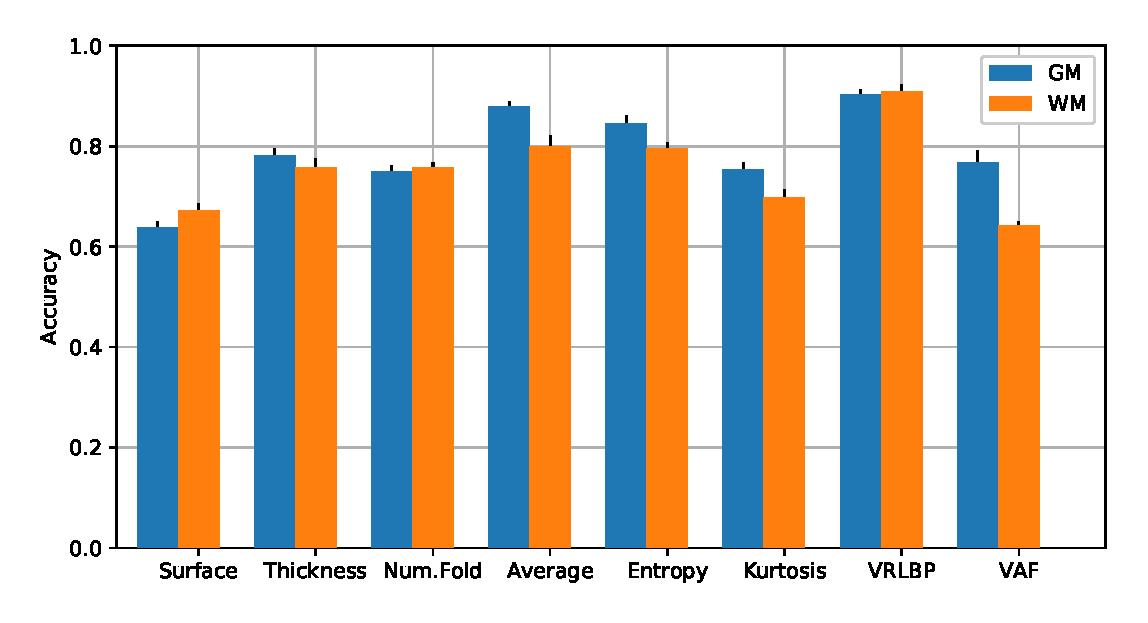
\includegraphics[width=0.9\columnwidth]{Graphics/ch6/12-performance}
	\caption{Performance at the operation point for the different mappings over the Grey Matter and White Matter, compared with the performance of \ac{VAF}.}
	\label{fig:performance}
\end{figure}

The first three approaches, Surface, Thickness and Number of Folds are easily interpreted, as they intend to represent the surface of the tissue by mapping the distance between the centre of the image and the last voxel, the thickness of the tissue, and a measure of the complexity of the different sulci and gyri. 

Surface and Thickness are highly related to other measures provided by widely-used software. However, as they are related to our more general \ac{SBM} description, their performance is poor, specially in the case of the Surface mapping. As it can be seen in Fig.~\ref{fig:masksGM}, and later in the $t$-maps at Fig.~\ref{fig:tmaps}, the detail of the surface map lacks higher detail, specially due to the superposing gyri and sulci. These superposition occur to a lesser extent in \ac{WM} tissue, and this is probably why this technique obtains higher performance in \ac{WM} than in \ac{GM}. 

As for the case of Thickness, although similar, it gathers much more information than the surface, without achieving, however, the level of detail of the cortical thickness measures provided by Freesurfer \cite{Fischl2004} or other software. Nevertheless, cortical thickness it is a descriptive, widely accepted as a measure of neurodegeneration in Alzheimer's Disease in the literature \cite{han2006reliability,Fischl2004}, and its measures might be relevant for a subsequent analysis. 

Number of Folds, however, is intended to model the complexity of the cerebral cortex, and therefore, it is of far more use in the case of \ac{GM} than in the \ac{WM}. This can be easily checked when looking at the maps obtained for both \ac{GM} and \ac{WM} in Figure~\ref{fig:masksGM}. 

The last three measures described in Section~\ref{sec:mapping} are statistical values that describe the variability of the sampling set $V_{\theta,\varphi}$. It would be reasonable to expect the better performance to be linked to the mapping that better models the tissue atrophy. 

This is the case of the average of these intensities, which can be interpreted as the total amount of tissue, being therefore a good measure of the level of brain atrophy in each direction $(\theta,\varphi)$. The average maps show the best performance of all the measures proposed in Section~\ref{sec:mapping}, and is higher in \ac{GM} than in \ac{WM}. This is consistent with the literature, as atrophy mainly occurs in \ac{GM} tissues. 

Entropy is a more complex statistical concept that comes from information theory, but is usually related to the amount of information, or in other words, the ``randomness'' of a source. In our particular case it could be interpreted as a measure of texture, that is, the grey-level variability in the direction of $\mathbf{v}_{\theta,\varphi}$. These maps perform very similar to the average ones in both \ac{GM} and \ac{WM}, suggesting that the entropy accounts for the tissue density as well. 

The last mapping defined, Kurtosis, is a fourth-order statistic, often interpreted as the peakedness (width of peak) of a probability distribution. In our context, it is related to the sharpness of the changes in the direction of $\mathbf{v}_{\theta,\varphi}$, and thus is related to the number of folds. As in the case of the latter, the Kurtosis performs poorly in both types of tissues, probably because they are measures that are not as directly related to atrophy as other measures such as average, entropy or thickness. 

The last of the single measures proposed in this work is the Volumetric Radial LBP defined in Section~\ref{sec:vrlbp}. It is a measure of the texture not only in the direction of $\mathbf{v}_{\theta,\varphi}$, but also in the neighbourhood of the mapping vector. Therefore, it is not strange that it obtains the best performance of the whole work, yielding accuracy results above $0.9$ for both \ac{GM} and \ac{WM} tissues. 

This could seem counter-intuitive, as the $t$-maps for this technique, presented in Fig.~\ref{fig:tmapvrlbp}, show small regions of high significance, when compared to the measures in Sec.~\ref{sec:mapping}. Yet, despite its size, it performs fairly well with a relatively small amount of data. It is probably due to the nature of VRLBP, and the areas highlighted in Fig.~\ref{fig:tmapvrlbp} probably correspond to the texture changes associated to the loss of tissue in the Hippocampus. 

As for the layered extension, which might seem a powerful method to add detail to the mappings, obtains however similar performance to the methodology above. It seems that the amount of information that can be obtained by each measure does not depend on the number of layers, and accordingly, its benefits are only related to visualization. In this case, best values are obtained in layer 2, which is consistent to the presence of some organs, specially the Hippocampus.  
%%%%%%%%%%%%%%%%%%%%%%%% 

\begin{figure*}[htp]% ROC
	\centering
	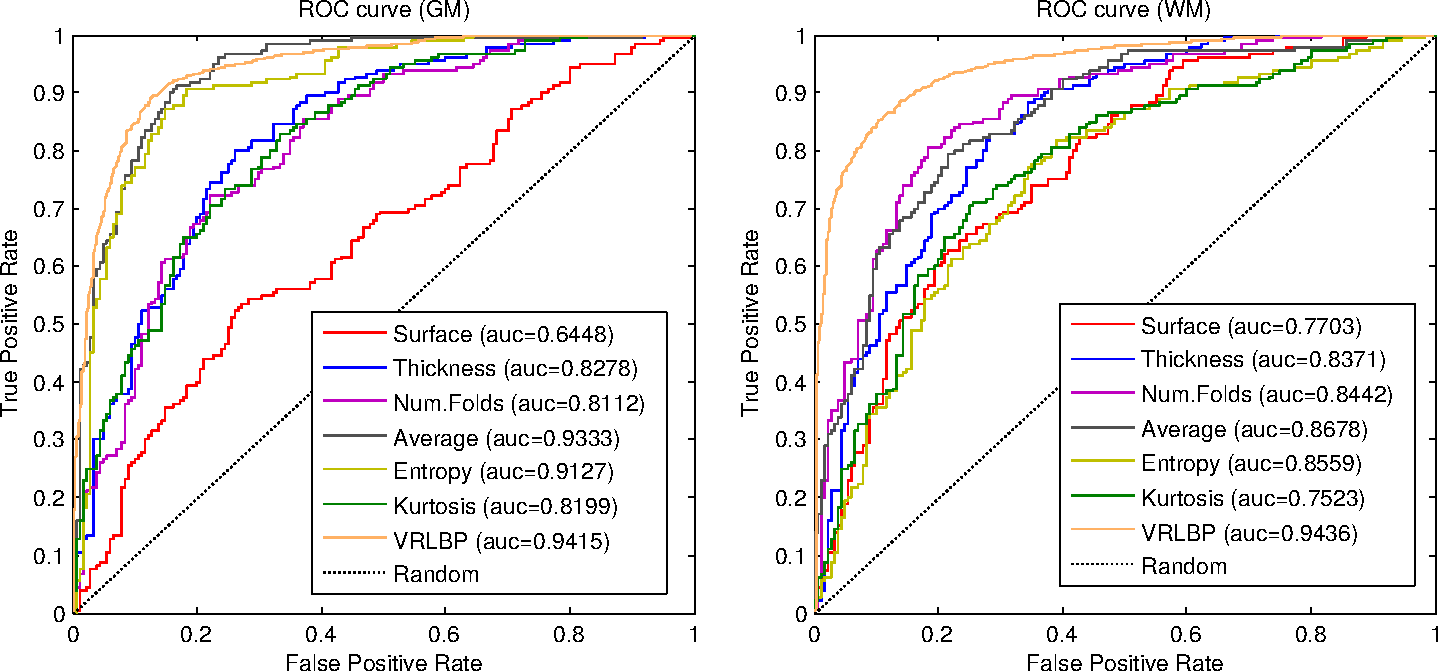
\includegraphics[width=0.8\textwidth]{Graphics/ch6/13-ROC}
	
	\caption{ROC curves of the different mappings for the \ac{GM} and \ac{WM} tissues.}
	\label{fig:roc}
\end{figure*}

Finally, in order to have another look at the performance of our mappings, the ROC curves of each type are presented in Figure~\ref{fig:roc}. There we can see how the VRLBP approach outperforms all the other measures, specially in the case of \ac{WM} tissue. In \ac{GM}, Average and Entropy present values really close to VRLBP, as expected. Conversely, the poorest performance is achieved by the Kurtosis and Surface mappings, however the Surface performs better in \ac{WM} than in \ac{GM}. These results confirm the performance values presented in  Table~\ref{tab:perfProj} and Figure~\ref{fig:figureGM}, making our proposed mapping framework a reasonable choice for obtaining both a visual interpretation of otherwise hidden features and a significant dimensionality reduction. 

It is important to note that our Spherical Brain Mapping defines a whole framework that can be easily extended with different sampling strategies. This is the case of the layered extension and the helical sampling in VRLBP, but they are only two examples of what can be done. 
Since our simplest approach implies a computation of a value from a vector of intensities, measures used to describe time-course data could be added to complete and highlight different properties of the tissues. In this context, high-order statistics \cite{Zhou2008}, as well as spectral measures \cite{Locatelli1998} have been successfully applied to analyse electroencephalogram (EEG) signals, and could be therefore applied here to bring different structural properties of the images into focus. 
Additionally, our mapping method is potentially applicable to other imaging modalities, such as PET and SPECT, where the structural information is sometimes lost \cite{IAIllan2010,Ram'irez2009}. Our technique does not need the use of complex co-registering of MRI and functional imaging to locate cerebral structures, as it rely only in their angle and depth. Moreover, in the case of Diffusion Tensor Imaging (DTI), which has proven itself as a good tool for the diagnosis of Alzheimer's Disease \cite{Grana2011,Medina2008}, \ac{SBM} could be modified to replace $\mathbf{v}_{\theta,\varphi}$ with each tract, and subsequently project a given feature, resulting in a summary of the tract's behaviour in a single two-dimensional image. 

			

\subsection{Paths via \ac{HMM}}\label{sec:discussion}
In this work we propose a new path tracing algorithm based on Hidden Markov Models used to trace similar intensity paths inside the brain. The paths are meant to be used as a feature extraction tool in the \ac{SBM} framework either by selecting voxels or computing features. We have performed several experiments to evaluate these approaches in a differential diagnosis of AD using MRI brain images. 

Our paths are defined so that they construct a minimum intensity variation path starting at the AC and oriented in a general direction set by the spherical coordinate pair $(\varphi,\theta)$. As commented before, the AC is the obvious starting point, given its privileged position in the middle of the left and right hemispheres. A different starting point will reveal suboptimal, stopping at disconnected regions such as the ventricles, and yielding incomplete paths. 

The paths adapt to the intensity changes in a certain direction in the brain, modelling grey level connectivity in all spherical directions. Since grey level is directly related to tissue density, we can assume that the outcome follows smooth, same-density paths that start in white matter and progressively transition to grey matter in a specific direction. Therefore, they are not functional connectivity maps like Diffusion Tensor Imaging (DTI), which have been used as well in the diagnosis of AD\cite{Grana2011,Medina2008}. While DTI fibers are the result of a tensor processing over diffusion images that quantify the water molecule motion -in both direction and average magnitude- at the voxel level, our \ac{HMM} paths only characterize grey level connectivity in static MRI images, and are meant to be used for feature selection. 

\begin{figure}
	\begin{center}
		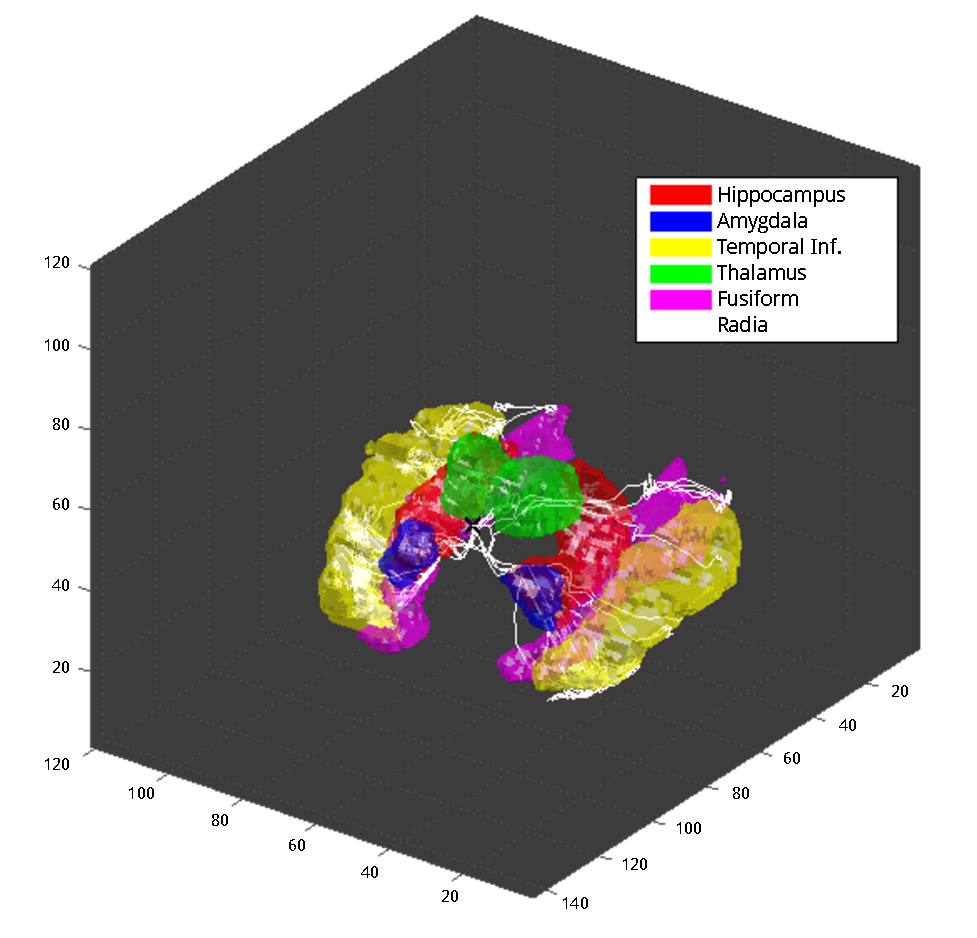
\includegraphics[width=\columnwidth]{Graphics/ch6/radia&structures}
		\caption{Paths that obtain more than 75\% accuracy, and a three-dimensional representation of the structures crossed by them.}
		\label{fig:bestPaths}
	\end{center}
\end{figure}

Our first experiment uses \ac{HMM} paths computed on the DARTEL template to describe how the intensity of the set of voxels corresponding to a certain path can be used as discriminant features in a SVM classifier. The differences in the distribution of intensities between controls and AD affected subjects are used to identify structural changes in AD. Fig.~\ref{fig:bestPaths} depicts the paths that achieved best performance (accuracy higher than $0.75$) in this differential diagnosis, superimposed to some structures rendered from the Automated Anatomical Labeling (AAL) brain atlas\cite{Tzourio-Mazoyer2002}.

The paths that obtained higher accuracy are those that cross structures such as the Hippocampus, Amygdala, Thalamus, Fusiform and Inferior Temporal Gyrus. Particularly, grey matter loss in the Hippocampus has been described in the NINCDS-ADRDA criteria for AD diagnosis\cite{Dubois2007} and is widely accepted\cite{chan2001patterns,Baron2001,Jong2008}. Furthermore, the evidence suggest that atrophy affects the surrounding structures (Amygdala, Parahippocampal and Fusiform Gyrus) as well\cite{chan2001patterns,Baron2001}. Some studies have found significant atrophy in the Thalamus and Putamen in early AD\cite{Jong2008} as well. Generally, in advanced AD, most of the neocortex and grey matter suffer from atrophy\cite{chan2001patterns,Baron2001,Jong2008}, which explains why most of the paths that involve the neocortex in Fig.~\ref{fig:accuracyMap} obtain accuracy rates around $0.7$. 

A number of feature maps have been computed as well. These are the result of applying some of the \ac{SBM} measures to the voxels selected by the \ac{HMM} paths. Variance and kurtosis have been proved as the most discriminative maps (with accuracy higher than $0.7$). This is coherent with the definition of the paths, where the intensity transitions are minimal. Therefore, average would be the less discriminative in this case, being higher order statistics such as variance or more representative of the tissue density distribution of each class. 

Regarding texture analysis, we have again discriminative features (with accuracy that surpass the 70\%) yet not very powerful. This situation might be due to the definition of the paths as minimum intensity variation paths, being the textural changes along the path minimal.  

However the real utility of these texture features could be in its application to longitudinal studies, since textsure can be related to evolution of the disease\cite{sikio2015mr}. It is very convenient to use a scalar to characterize a measure (in our case, texture features) in each direction. The texture obtained in each session can be used to construct a function of neurodegeneration that allows the exploration of the different stages of the disease as the changes in the brain texture along the time within a single patient. 

Table \ref{tab:comparison2} presents some of the best results of our methodology involving \ac{HMM} paths in this order: the performance of a single path and using the selected paths as features (Section~\ref{sec:intensity}), the performance of using projected maps (in this case, variance and kurtosis) like in the \ac{SBM} paper (Section~\ref{sec:intensity}) and the results of computing texture maps using radial GLCM and Haralick Texture Features (Section~\ref{sec:texture}). It is compared with the methods using in the \ac{SBM} paper\cite{Martinez-Murcia2015}, the \ac{SBM}-VRLBP\cite{Martinez-MurciaVRLBP}, the \acf{VAF}\cite{Stoeckel04} algorithm and different approaches used in the ADNI database and involving SVM classifiers such as the LVQ-SVM\cite{Ortiz2013} or Spatial Component Analysis (SCA)\cite{Illan2014}. 

\begin{table*}
	\myfloatalign
	\begin{tabularx}{\textwidth}{Xccc}
			\tableheadline{Feature} & \tableheadline{Accuracy} & \tableheadline{Sensitivity} & \tableheadline{Specificity} \\ \midrule
			Paths & $0.806 \pm 0.069 $ & $0.733 \pm 0.073$ & $0.878 \pm 0.097$\\
			Selected Paths & $0.828 \pm 0.054 $ & $0.794 \pm 0.095$ & $0.861 \pm 0.039$\\
			Variance & $0.750 \pm 0.064 $ & $0.633 \pm 0.131$ & $0.867 \pm 0.102$\\
			Kurtosis & $0.756 \pm 0.105 $ & $0.733 \pm 0.165$ & $0.778 \pm 0.150$\\
			Texture (Difference Variance) & $0.736 \pm 0.070 $ & $0.683 \pm 0.098$ & $0.789 \pm 0.090$\\
			\midrule 
			\ac{VAF}  & $0.768 \pm 0.011$ & $0.752 \pm 0.016$ & $0.785 \pm 0.016$ \\
			\ac{SBM}-average (\ac{GM})  & $0.879 \pm 0.005$ & $0.897 \pm 0.006$ & $0.861 \pm 0.006$ \\
			\ac{SBM}-average (\ac{WM})  & $0.800 \pm 0.011$ & $0.802 \pm 0.013$ & $0.798 \pm 0.009$ \\ 
			\ac{SBM}-VRLBP (\ac{GM})  & $0.903 \pm 0.010$ & $0.890 \pm 0.012$ & $0.916 \pm 0.018$ \\
			\ac{SBM}-VRLBP (\ac{WM}) & $0.909 \pm 0.014$ & $0.899 \pm 0.028$ & $0.919 \pm 0.018$ \\
			LVQ-SVM (\ac{GM}) & $0.869 \pm 0.101$ & $0.822\pm0.120$ & $0.890\pm0.102$ \\ 	
			SCA (\ac{GM}) & $0.880 \pm0.0^* $ & $0.926\pm0.0^* $ & $0.845\pm0.0^*$ \\ 
			SCA (\ac{WM}) & $0.808 \pm 0.0^*$ & $0.817\pm0.0^*$ & $0.800\pm0.0^*$ \\ 	
			\bottomrule
			\multicolumn{4}{l}{$^*$ SCA used leave-one-out cross-validation. SD is 0.}
		\end{tabularx}
		
		\caption{Comparison between our algorithm performance values (best values for selected voxels in all paths and texture features) ($\pm$SD) and other methods in the bibliography} \label{tab:comparison2}
	\end{table*}
	
	
	\ac{VAF} is often used as a baseline when comparing different methodology, as it has been described as a good estimator of the accuracy obtained by means of visual analysis \cite{Stoeckel04}. As we commented before, the raw voxel intensities selected by our DARTEL paths achieve higher accuracy than statistical or texture features, and it is the only strategy that outperforms \ac{VAF}. Texture and statistical features obtain poorer, although still good, performance (around 75\% accuracy). When compared to other methods, the difference is greater, although inside the range of 1 SD. Most of the \ac{SBM} features proposed in \cite{Martinez-Murcia2015} perform better than our DARTEL paths, and the case of \cite{Martinez-MurciaVRLBP} even surpass the barrier of 90\% accuracy. However, there is a significant difference with these approaches, and it is that these measures used segmented \ac{GM} and \ac{WM} images, instead of using the whole MRI. Segmentation, thus, enhances the detection and extraction of features from the images, whereas the tracing of paths over the whole images is a more complex operation. When compared to LVQ-SVM or SCA, the difference in performance is even smaller and still inside the range of 1 SD, which gives us an idea of the ability of our methodology to detect patterns with a significant feature reduction.
	
	Finally, one might argue if a different approach to the path tracing, such as tracing the set of paths in each subject individually might be of use. This strategy would still characterize the individual brain structure; however the way this structure is defined would be different: the spatial location of the nodes and topology of the paths instead of the intensity distribution. Given the time our algorithm takes to model one single MRI (around 2 hours) it can be extraordinarily computationally expensive, although faster than other methodology like DTI fiber tracing or Freesurfer surface extraction. Consequently, it would be an interesting option to explore in future works. 